\documentclass[uplatex, dvipdfmx, a4paper, report, papersize, 11pt]{jsbook}
\usepackage{bm}
\usepackage{amsmath}
\usepackage[dvipdfmx]{graphicx}
\usepackage{wrapfig}
\usepackage[hang, small, bf]{caption}
\usepackage[subrefformat=parens]{subcaption}
\usepackage{here}
\usepackage{comment}
\captionsetup{compatibility=false}

\bibliographystyle{junsrt}
\title{二色の光周波数コムによるレーザー冷却法の開拓}
\author{物理工学科4年 中西亮}
\date{2018/11/19}
\begin{document}
\maketitle
\newpage

\setcounter{tocdepth}{2}
\tableofcontents

\newpage
\chapter{光周波数コムのテーパーアンプによる増幅実験}

\section{光周波数コムのテーパーアンプによる増幅}
 第3章の議論から分かる通り、二色のコムによるCs原子の冷却を行うに当たり、数十から数百ミリワットのコムを$760$ nm付近と$894$ nm付近で用意する必要がある。しかし、現在当研究室が所有する光周波数コムから上記の周波数帯を切り出したときの、平均パワーは一ミリワット程度しかない。そのため今回の実験では、光周波数コムから得られた光をテーパーアンプ(Tapered Amplifier,  TA)を用いて増幅するという手段を用いる。しかし、通常TAはcwレーザーを増幅するために用いられるため、光周波数コムの増幅に用いた場合にどのような振る舞いを見せるかについての過去の研究は限られており、異なる繰り返し周波数に対してのTAの増幅の振る舞いを調べた研究はまだない。今回の実験では繰り返し周波数の異なる光周波数コムに対してTAの増幅の様子を測定した。

\section{テーパーアンプの原理}
今回の実験では光周波数コムの光をTAで増幅しているが, この節ではTAの原理について説明する.

\subsection{半導体レーザーの発光原理}
TAは半導体で構成されており, その発光原理は半導体レーザーと同様であり構造も非常に似通っている. このため, まず文献\cite{わかる半導体レーザーの基礎と応用}の議論に沿って, 半導体レーザーの発光原理について説明する. 半導体レーザーの基本構造は図\ref{semicon_structure}のように, 3層のサンドイッチ構造で出来ており, 真ん中に挟まれ発光する層を「活性層」, 活性層を挟み込んで光やキャリアを閉じ込める役割を担う二つの層を「クラッド層」と呼ぶ. このような構造をDH(Double Hetero)構造と呼ぶ.\\
 この半導体p-n接合のエネルギーバンド構造は図\ref{semicon_bands}のようになる. 半導体レーザーでは図\ref{semicon_bands}のように電子が伝導帯から価電子帯に落ちる際のエネルギー差に相当する光が放出されるが, バンド間遷移であるためにライン間遷移に比べ発光スペクトルは広い. この素子に図\ref{semicon_structure}のように順方向のバイアスをかけるとエネルギーバンドが平らになっていき, p-n接合領域に電子とホールが集まり反転分布が形成される. このバンドギャップはGaAsの場合, 約$1.4$ eVで$800$ nmから$900$ nmに相当する\cite{grynberg_aspect_fabre_cohen-tannoudji_2010}. 半導体レーザーでは活性層の両へき界面に鏡をコーティングすることで光フィードバックを実現しレーザー動作を可能としている.

\begin{figure}[htpb]
  \centering
    \begin{tabular}{c}

%----- 半導体レーザーの構造 -----

      \begin{minipage}{0.70\hsize}
        \centering
          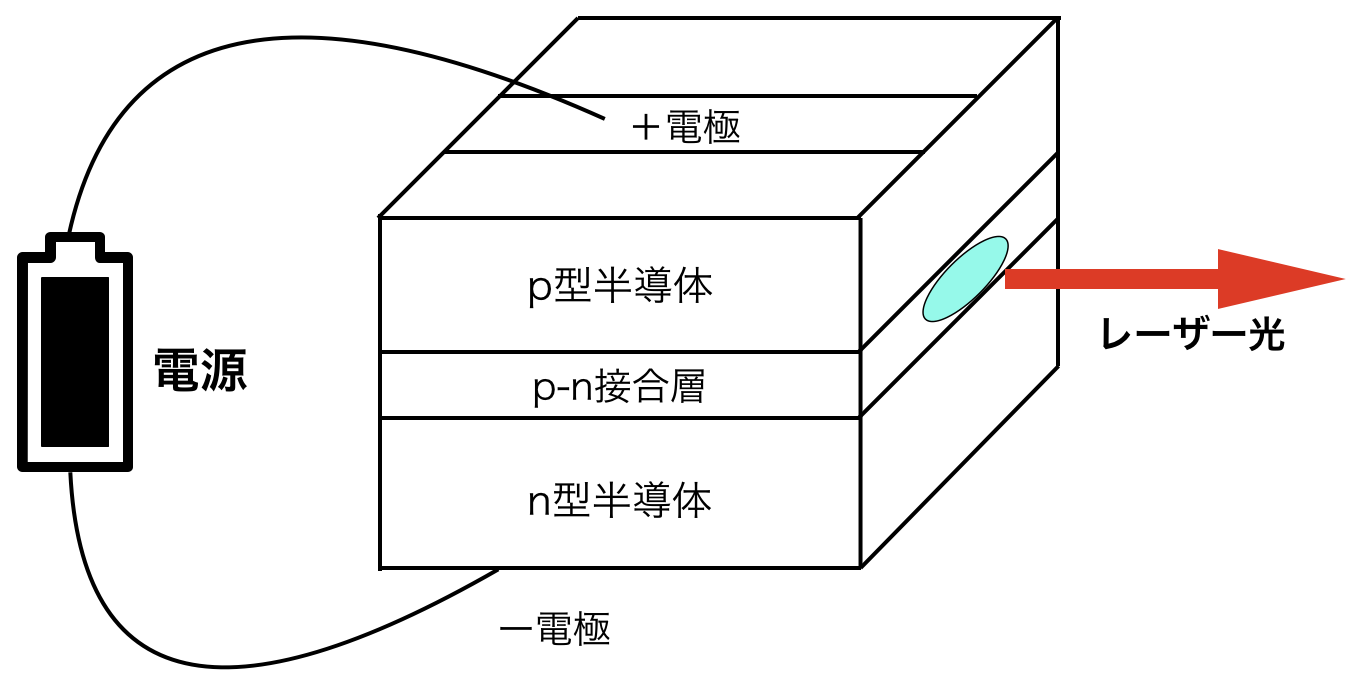
\includegraphics[keepaspectratio,  scale=0.35,  angle=0]
                          {figures/chapter2/semicon_structure.png}
                          \caption{半導体レーザーの基本構造}
                          \label{semicon_structure}
      \end{minipage}\\
      \\
      \\

%----- バンド図 -----

      \begin{minipage}{0.70\hsize}
        \centering
          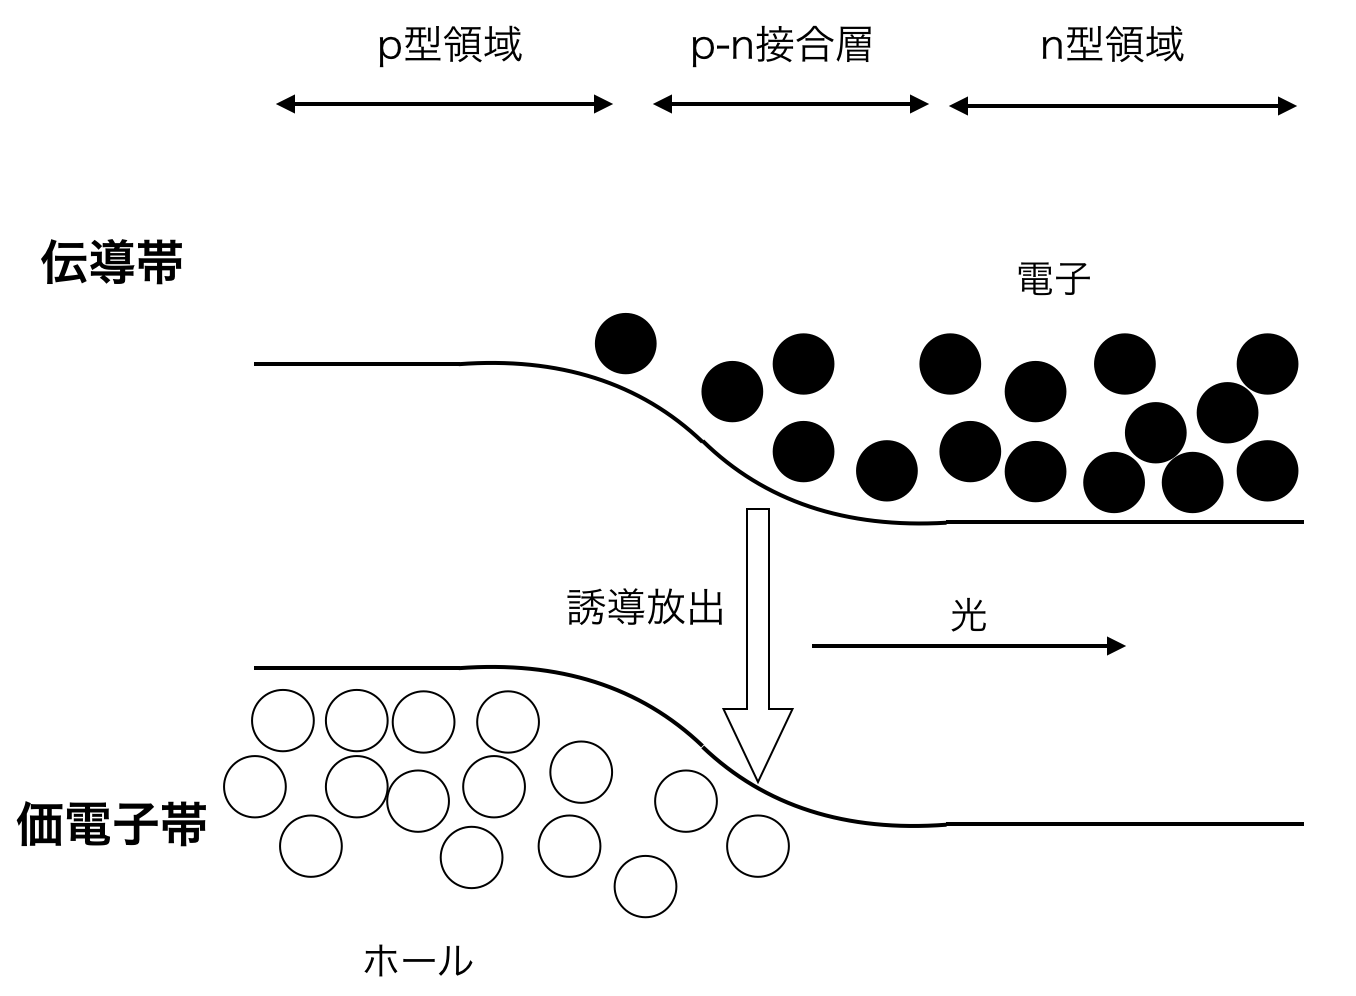
\includegraphics[keepaspectratio,  scale=0.30,  angle=0]
                          {figures/chapter2/semicon_bands.png}
                          \caption{半導体レーザーのバンド図}
                          \label{semicon_bands}
      \end{minipage}

  \end{tabular}
\end{figure}
\newpage

\subsection{テーパーアンプ}
 TAは近赤外の連続波(continuous wave,  cw)のレーザーを$20$ dB以上の利得で増幅することができる素子として知られている\cite{Cruz:06}.\\
 TAは図\ref{TA_structure}のような構造をしており, 半導体レーザーと同じDH構造を有している. TAの特徴は入力側から出力側にだんだんと拡がっているゲイン領域である. また, 増幅器として用いるためへき界面に反射材がコーティングされておらず光フィードバックがないことが半導体レーザーとの大きな違いである.\\
 TAの一つの特徴は従来の細いストライプを持つ半導体レーザーよりも高い輝度を出せることである. 輝度は
 \begin{equation}
   B = P/(A\Omega)
 \end{equation}
で定義される. ただし, Pは光の出力パワー, Aは放出面積, $\Omega$は光の放出される立体角を表す. 輝度は, レーザーの空間モードが一つであるとき, およそ
\begin{equation}
  B = P/\lambda^2
\end{equation}
の最大値をとる\cite{Walpole1996}. ただし, $\lambda$は波長を表す. このようなレーザーのビームを回折限界であるという. 従来の幅の細いゲイン領域ではバルクや発光面の加熱効果によって得られるパワーが数百ミリワットに限られていた. また, より幅のあるゲイン領域を用いると横モードを一つに保つことが難しいという欠点があった.これに対して, cwレーザーをTAを用いて増幅した場合, 数ワットの回折限界の出力を得ることができる\cite{Walpole1996}.


\begin{figure}[htbp]
 \begin{center}
  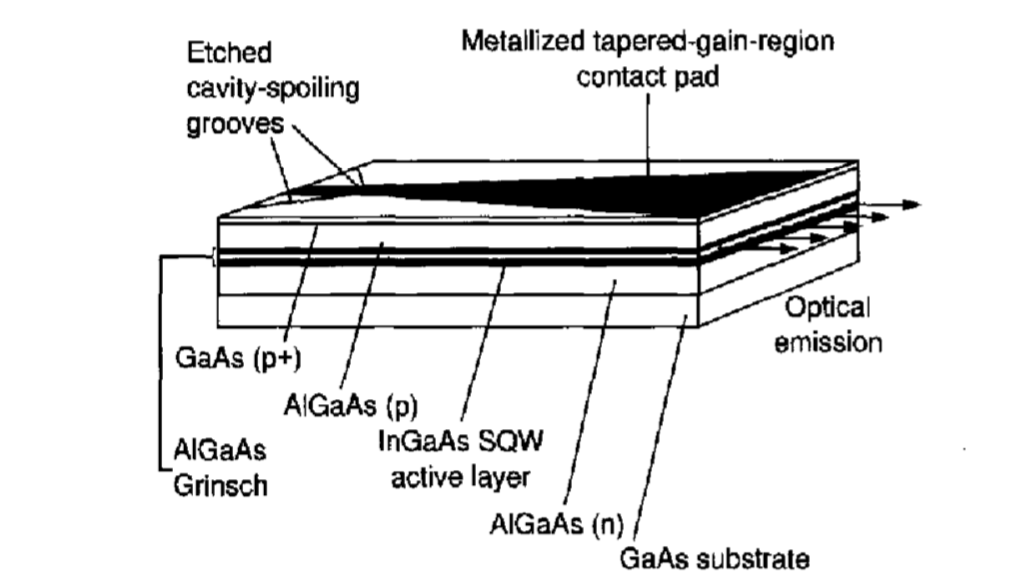
\includegraphics[width=100mm]{figures/chapter2/TA_structure.png}
 \end{center}
 \caption{TAの基本構造(文献\cite{Walpole1996}から引用)}
 \label{TA_structure}
\end{figure}


\newpage
\section{繰り返し周波数$120$ MHzのコムの$766$ nm付近の増幅}
\subsection{測定手法}
繰り返し周波数が$f_{\mathrm{rep}} = 120$ MHzのコムの、$766$ nmを中心波長とする幅$10$ nmのバンドパスフィルター(BPF)を通過した光をTAで増幅させ、マスター光とスレーブ光のパワーを測定した。その際に、BPF通過前のコムのスペクトルと、テーパーアンプの入り口と出口でのコムのスペクトルも測定を行った。その際の光学系は図\ref{760_amp_diagram}に示している。実験では最初にアイソレータを入れないでTAの実験を行ったところ、後述の通りTAからの戻り光がコムに光フィードバックをもたらしcw的発振を引き起こすことが観測された。このためアイソレータを使用している。

\begin{figure}[htpb]
  \centering
    \begin{tabular}{c}
      \begin{minipage}{1\hsize}
        \centering
          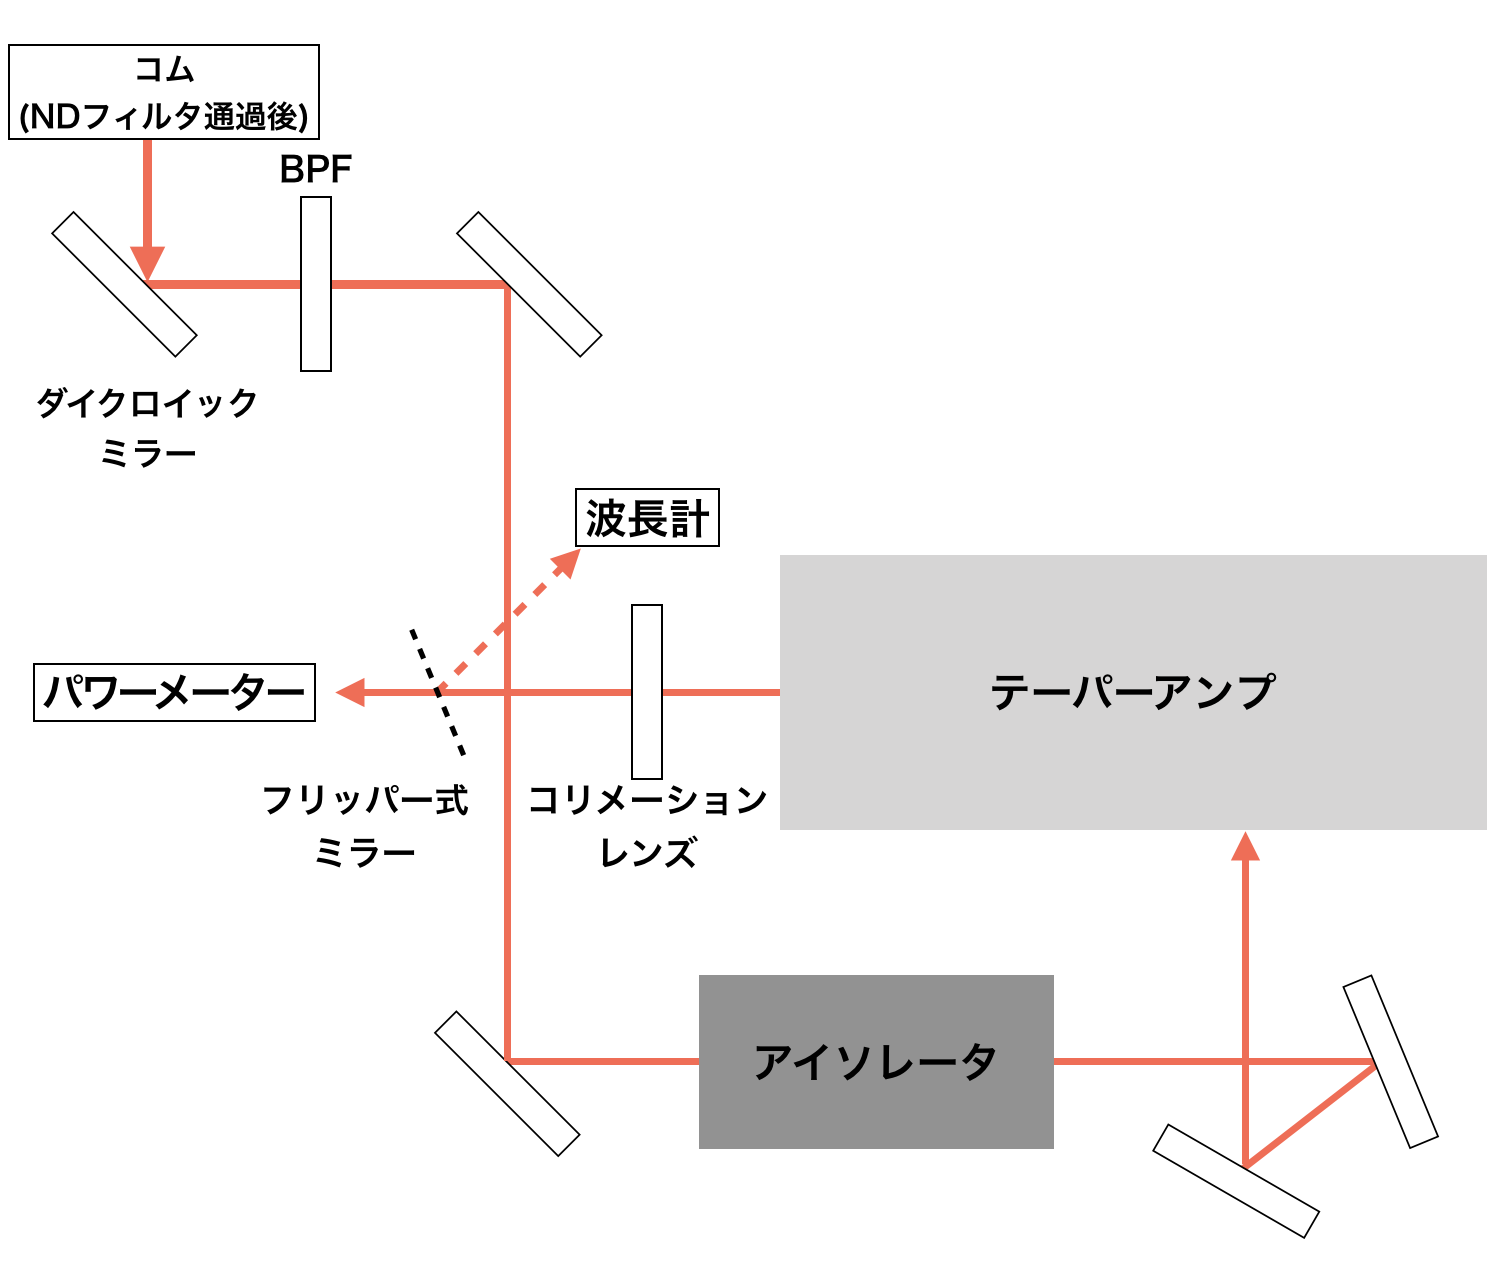
\includegraphics[keepaspectratio,  scale=0.4,  angle=0]
                          {figures/chapter4/760_amp_diagram.png}
                          \caption{繰り返し周波数$120$ MHzのコムの$766$ nm付近の光を増幅した際の光学系。まずアイソレータなしで測定し、その後アイソレータを設置して測定を行った。}
                          \label{760_amp_diagram}
      \end{minipage}
    \end{tabular}
\end{figure}

\subsection{測定結果}
\subsubsection{TAの戻り光による光周波数コムのスペクトルの変化}
 図\ref{spectrum_current_MODORI}はマスター光入射時にアイソレータを使用しなかった時の、光周波数コムのキャビティの出力口におけるスペクトラムをTAに印加する電流の大きさを変えつつ分光器で測定したものである。TAの印加電流をあげていくと$770$ nm付近でcw的な発振を起こしていることが分かる。これはTAの入射口から出た自然放出の光が光周波数コムの共振器まで戻り、光フィードバックを起こしているものと考えられる。\\
 そのためマスター光入射時にアイソレータを通過させたところ、スペクトルは図\ref{spectrum_current_isolator}のようになった。このようなcw的な発振は観測されなかった。
\begin{figure}[H]
 \begin{center}
  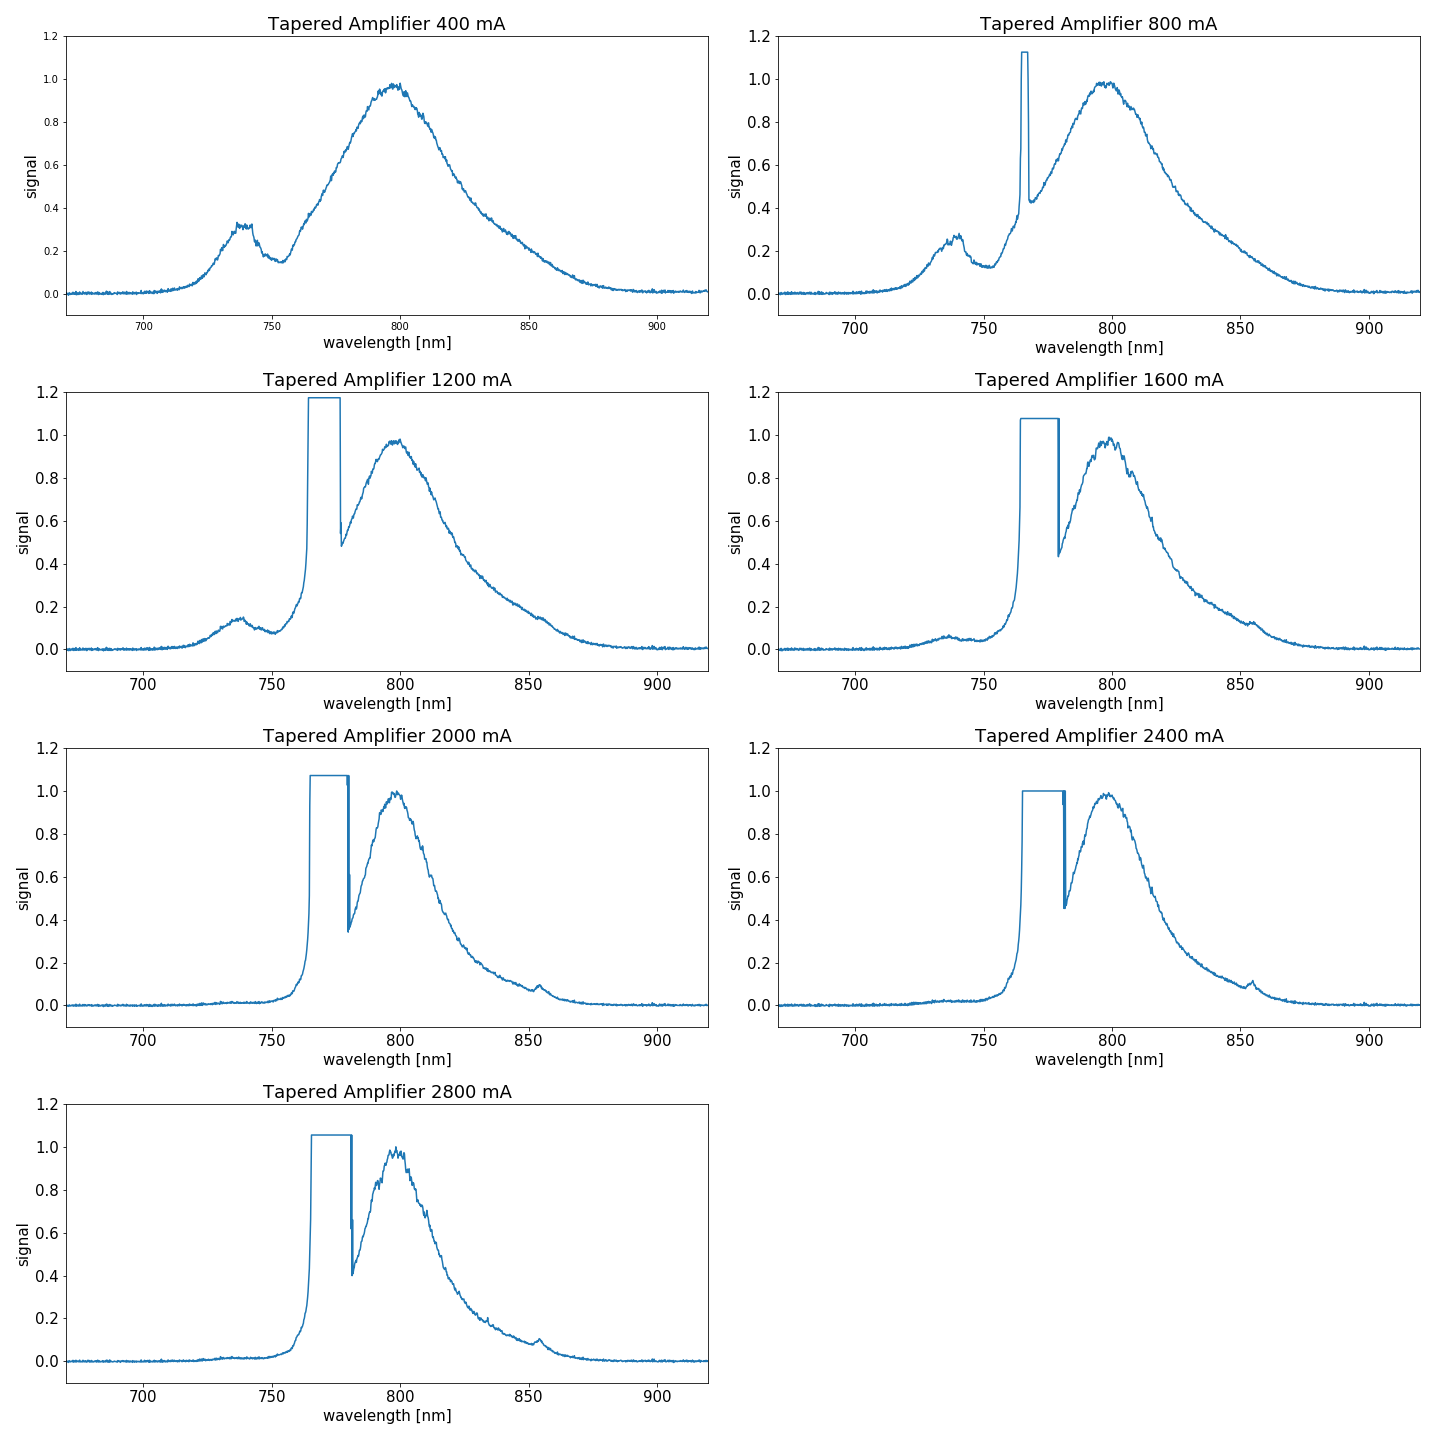
\includegraphics[width=140mm]{figures/chapter4/spectrum_current_MODORI.png}
\end{center}
 \caption{戻り光の影響によるコムのスペクトルのTAの印加電流依存性。$f_{\mathrm{rep}} = 120$ MHzのコムで$766$ nm付近の波長を増幅した時のコムの出力口から出た光の一部を測定した。}
 \label{spectrum_current_MODORI}
\end{figure}
\begin{figure}[H]
 \begin{center}
  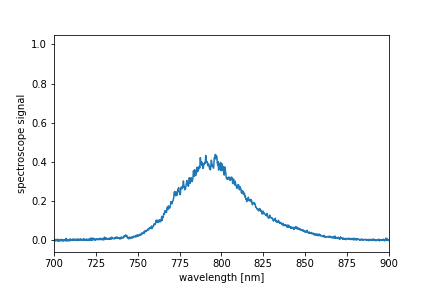
\includegraphics[width=100mm]{figures/chapter4/comb-spectrum_no-return.png}
\end{center}
 \caption{アイソレータ使用時のコムのスペクトル。$f_{\mathrm{rep}} = 120$ MHzTAのコムで$766$ nm付近の波長を増幅し, 印加電流は$1617$ mAとした。コムの出力口から出た光の一部を計測した。}
 \label{spectrum_current_isolator}
\end{figure}

\subsubsection{TAの増幅の振る舞いの測定結果}
 スレーブ光のパワーのマスター光のパワーによる変化は図\ref{766-M-S-power}のようになった。出力パワーからマスター光なしのときのパワーを自然放出のパワーとして差し引いた値をスレーブパワーとしている。これ以後の全ての実験でこの処理を行っている。また、その際のスペクトルの変化は図\ref{766_slave-input-power}に示した。また、スレーブ光のパワーとスペクトルのTAの印加電流による変化は図\ref{Gain-current-766,766_slave-current_spectrum}のようになった。\\
 図\ref{766-M-S-power}を見るとスレーブパワーは$15$ mW程度で飽和している様子が分かる。また、図\ref{Gain-current-766}を見ると印加電流に対しては$1400$ mW程度からやや傾きが小さくなっており飽和に近づいていると推測される。
 また、図\ref{766_slave-input-power}に示されたスレーブ光のスペクトルを見ると、マスターパワーが大きくなると出力のピーク付近の形状がややコムの波長分布を反映してピークが出るが、スペクトルの裾の部分の形状には大きな変化は見られないことがわかる。次にスレーブ光のスペクトルの電流依存性を示した図\ref{Gain-current-766}を見ると、やはりピーク付近のスペクトルの形状が電流が増えていくにしたがって、コムの形を反映したものになっていることがわかる。裾の部分の形状に大きな変化は見られない。
\begin{figure}[htpb]
  \centering
    \begin{tabular}{c}

      \begin{minipage}{0.50\hsize}
        \centering
          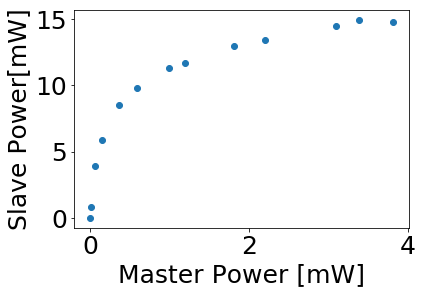
\includegraphics[keepaspectratio,  scale=0.45,  angle=0]
                          {figures/chapter4/766-M-S-power.png}
                          \caption{スレーブ光のパワーのマスター光のパワー依存性。$f_{rep} = 120$ MHzで766nm付近の波長を増幅した。}
                          \label{766-M-S-power}
      \end{minipage}
      \begin{minipage}{0.50\hsize}
        \centering
          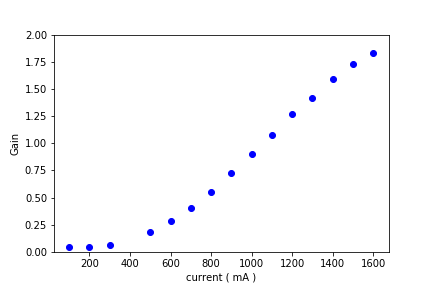
\includegraphics[keepaspectratio,  scale=0.5,  angle=0]
                          {figures/chapter4/Gain-current-766.png}
                          \caption{スレーブ光のパワーの印加電流依存性。$f_{rep} = 120$ MHzで766nm付近の波長を増幅した。}
                          \label{Gain-current-766}
      \end{minipage}
   \end{tabular}
\end{figure}

\newpage
\begin{figure}[H]
  \centering
    \begin{tabular}{c}
      \begin{minipage}{1\hsize}
        \centering
          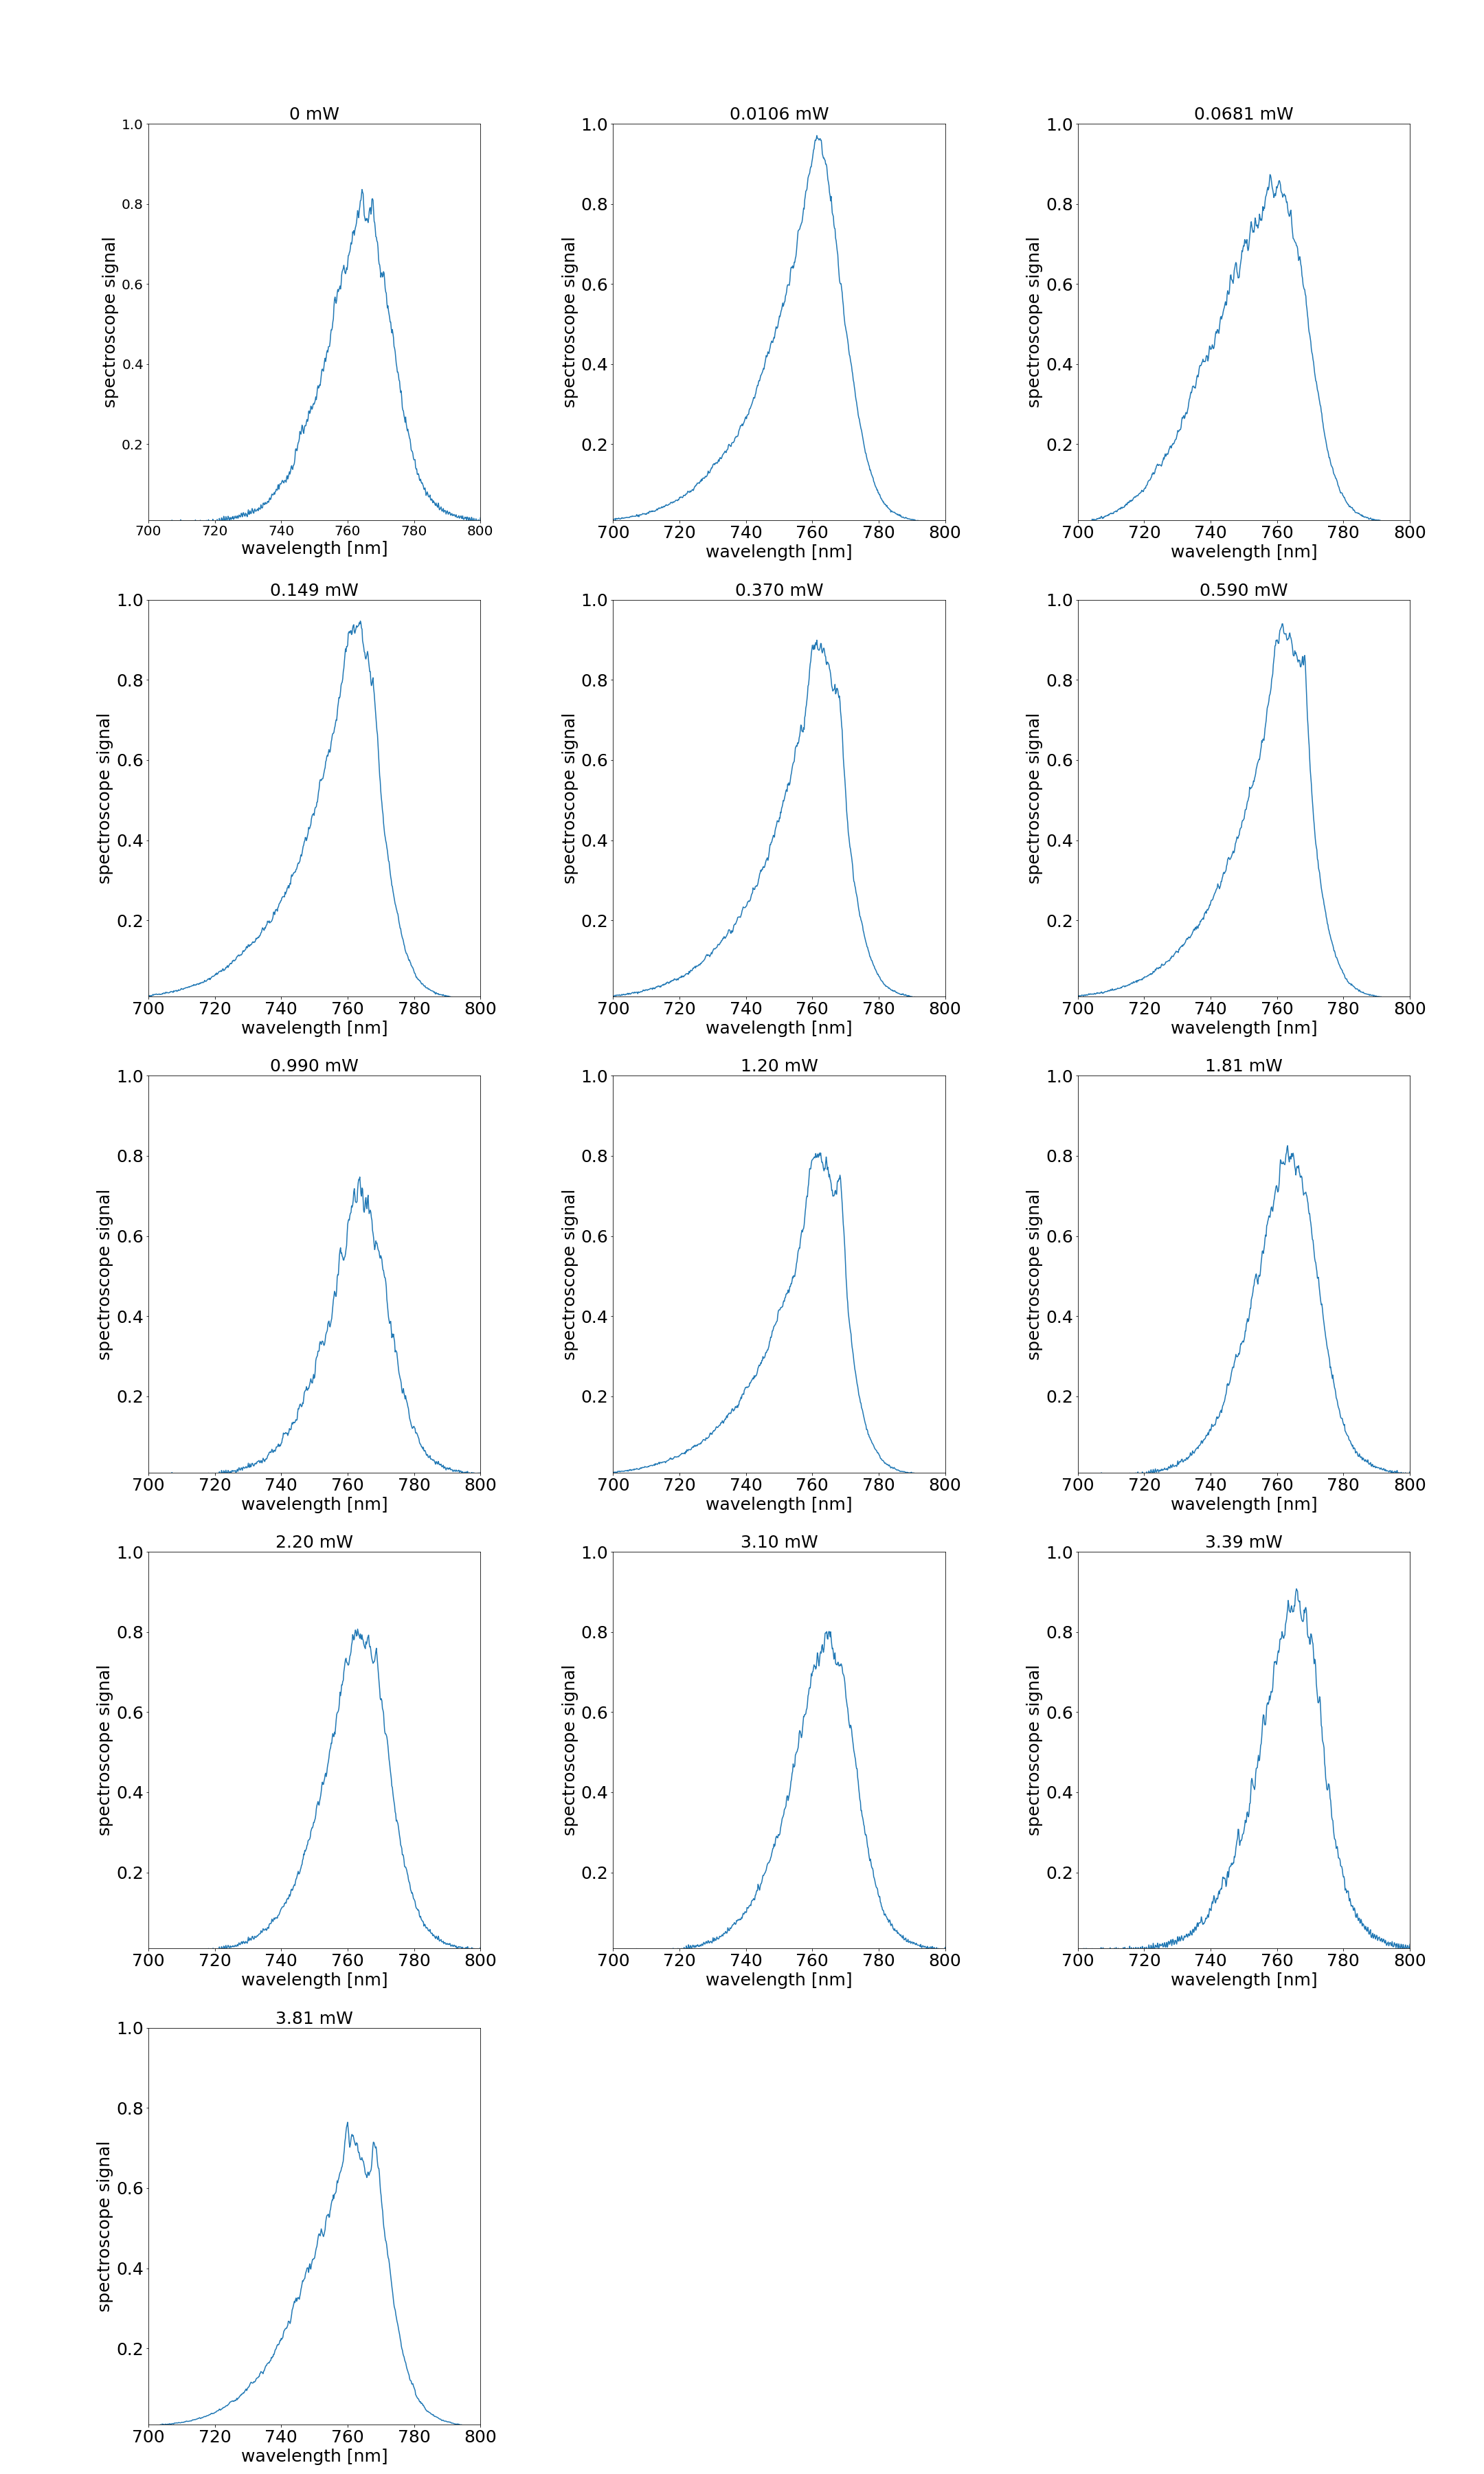
\includegraphics[keepaspectratio,  scale=0.15,  angle=0]
                          {figures/chapter4/766_slave-input-power.png}
                          \caption{スレーブ光のスペクトルのマスター光のパワー依存性}
                          \label{766_slave-input-power}
      \end{minipage}
  \end{tabular}
\end{figure}

\newpage
\begin{figure}[H]
  \centering
    \begin{tabular}{c}
      \begin{minipage}{1\hsize}
        \centering
          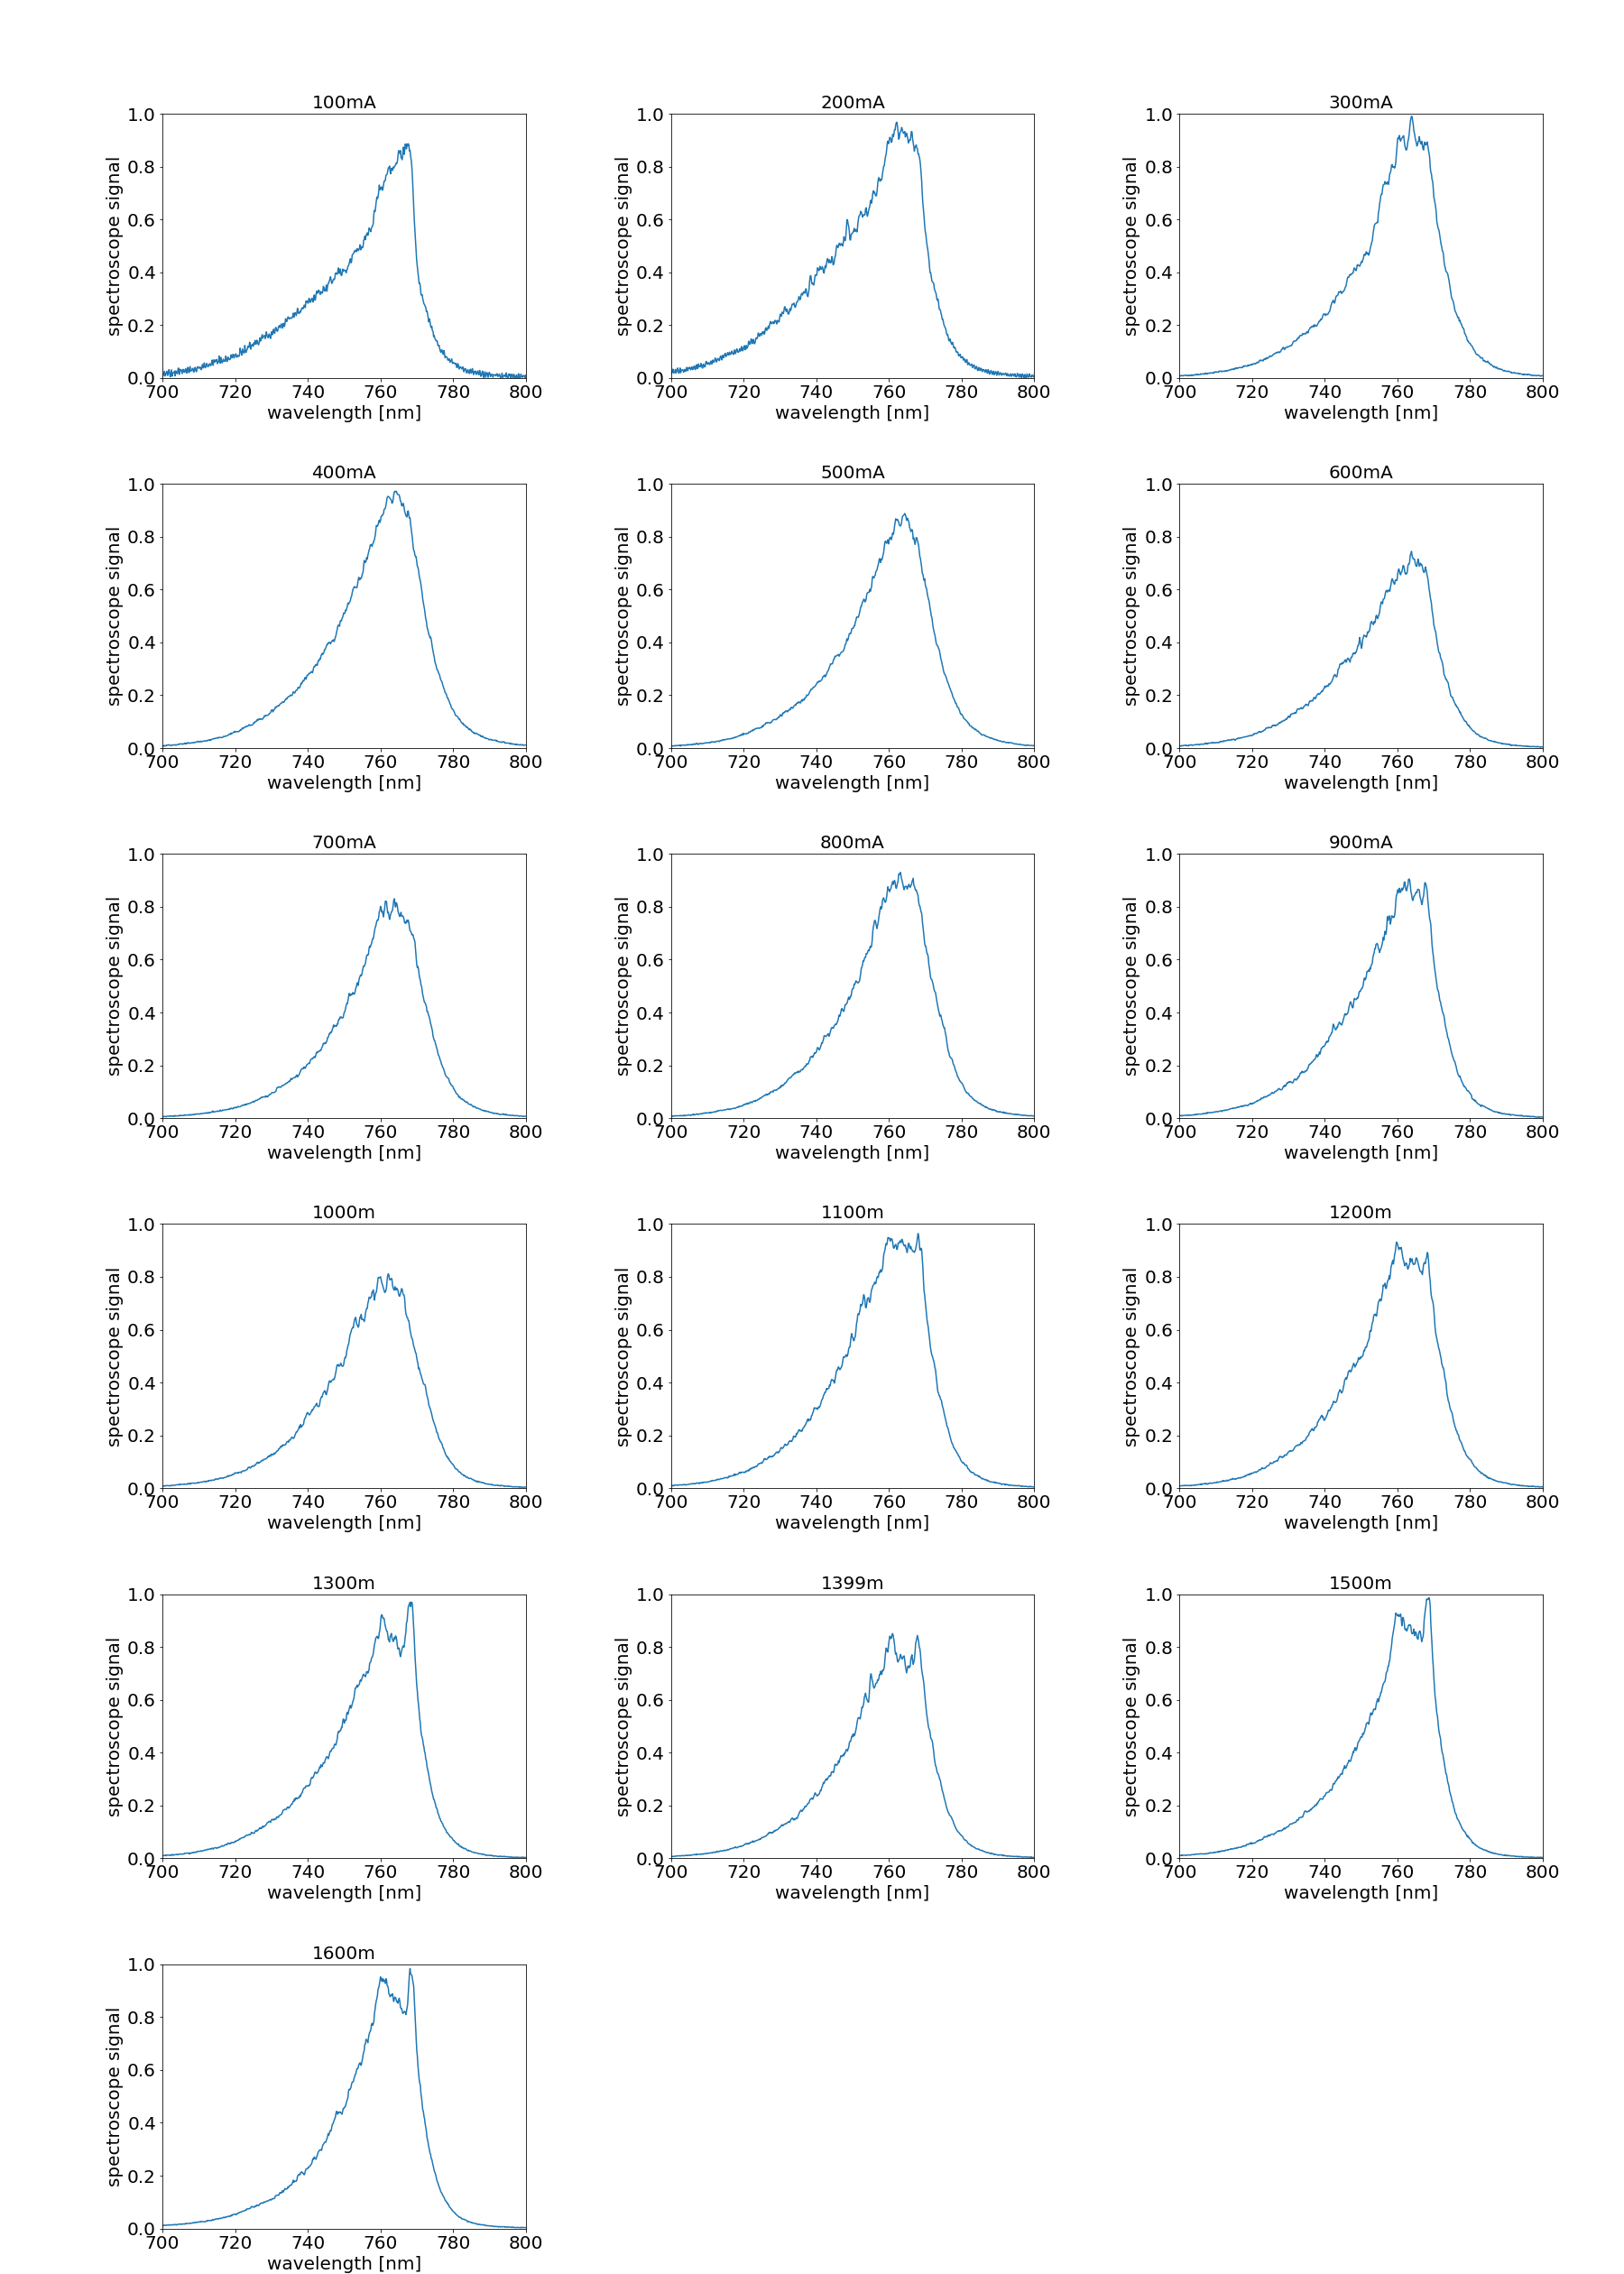
\includegraphics[keepaspectratio,  scale=0.20,  angle=0]
                          {figures/chapter4/766_slave-current_spectrum.png}
                          \caption{スレーブ光のスペクトルの印加電流依存性}
                          \label{766_slave-current_spectrum}
      \end{minipage}

  \end{tabular}
\end{figure}
\newpage

\subsection{考察}
\subsubsection{注入される電子数とレーザーの光子数による考察}
$f_{\mathrm{rep}} = 120$ MHzのコムでは利得の飽和が観測されたが、二光子冷却の励起効率を考えたときに必要なスレーブ光のパワーが得られていない。そこで、TAによるコムの増幅において利得を上げるためにはどのような手法が必要となるのかを簡単なモデルを用いて原理的に考察を行う。\par
図のような直方体のゲイン領域をもつ半導体の増幅素子を考える。この素子には電流$I$によってキャリアとホールが注入されており、これらの再結合によって光子を生成するメカニズムとなっている。このキャリアの再結合のプロセスにはマスター光による誘導放出に加えて自然放出や自然放出の光子による誘導放出など複数のものがあるが、これらを全てまとめた実効的なキャリアの寿命を$\tau$とする。このとき、キャリア密度$n_{\mathrm{c}}$の時間変化を表す微分方程式は
\begin{equation}
  \frac{dn_{\mathrm{c}}}{dt} = \eta \frac{I}{eV}-\frac{n_{\mathrm{c}}}{\tau}
\end{equation}
と書ける。ここで、$\eta$は量子効率、$e_0$は電気素量、$V$はゲイン領域の体積を表す。この微分方程式を初期条件$n_c = 0$の下で解くと
\begin{equation}
  n_c = \frac{\eta\tau I}{e_0V}\left(1-e^{-\frac{t}{\tau}}\right)
\end{equation}
キャリア密度の上限は印加電流の大きさとキャリアの寿命にによって決まることが分かる。キャリア密度の時間変化は図\ref{carrier_saturation}のようになるので、キャリア密度の飽和はキャリアの寿命程度の時間でおこることが分かる。\\
\begin{figure}[H]
 \begin{center}
  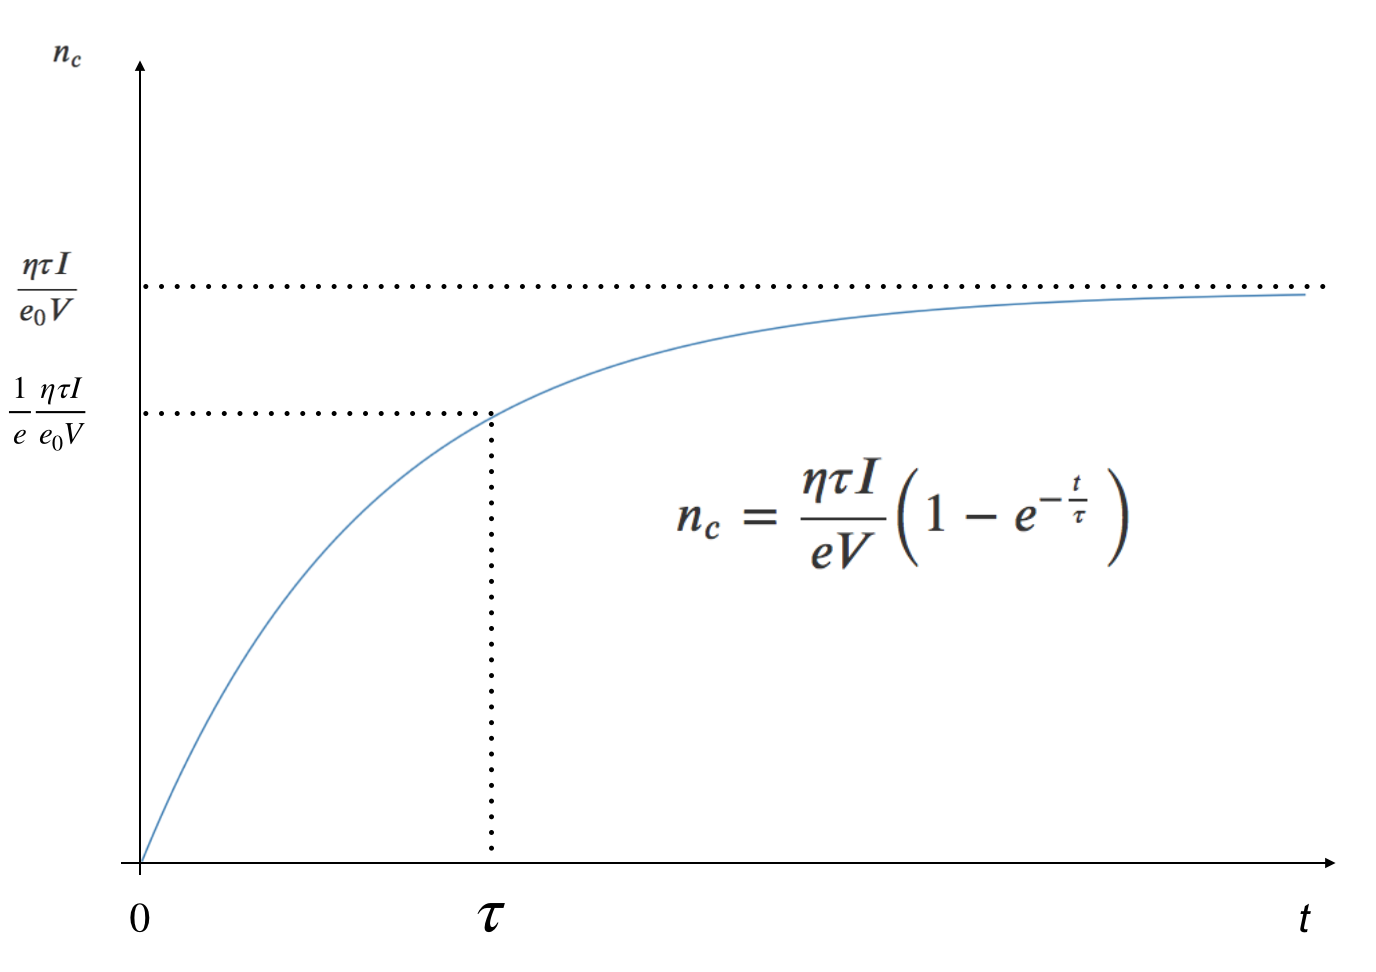
\includegraphics[width=100mm]{figures/chapter4/carrier_saturation.png}
\end{center}
 \caption{キャリア密度の時間変化}
 \label{carrier_saturation}
\end{figure}
cw光をTAで増幅した場合、通常$10$ mW程度のマスター光を$1$ A程度の印加電流で$1$ W程度まで増幅することができる。このとき、$766$ nmのスレーブ光に単位時間あたり含まれる光子数を計算すると、
\begin{equation}\label{TA_photon_rate}
  \frac{1\ \mathrm{W}}{1.6\ \mathrm{e_0V}\times1.6\times10^{-19}\ \mathrm{C}} = 4\times10^{18}\ 個\mathrm{/s}
\end{equation}
となる。これに対して$1$ Aの電流から毎秒含まれる電子数を計算すると、
\begin{equation}
  \frac{I}{e_0} = \frac{1\ \mathrm{A}}{1.6\times10^{-19}\ \mathrm{C}} = 6\times10^{18}\ 個\mathrm{/s}
\end{equation}
となる。両者を比較するとcw光のTAによる増幅においては注入された電子が効率よく光子に変換できていることが分かる。\par
これに対して、コムのパルスの増幅を行う場合を考える。キャリアの寿命を$500$ psと仮定するとこの時間でTAが供給できるフォトン数は式(\ref{TA_photon_rate})を用いると、
\begin{equation}
  4\times10^{18}\times500\times10^{-12} = 2\times10^9 個
\end{equation}
と計算できる。
 これに対して、$f_{\mathrm{rep}} = 120$ MHzのコムが$120$ mWの平均パワーを持つ時の一つのパルスのエネルギーは$10$ pJとなる。一つのパルスに含まれる光子の数は
\begin{equation}
  \frac{10\ \mathrm{pJ}}{1.5\ \mathrm{eV}\times1.6\times10^{-19}} = 4\times10^7 個
\end{equation}
となる。よってこの計算では増幅の利得は$50$倍程度となる。実際にはASEなどの効果でキャリアの寿命はより短くなると考えられるので、パルスに含まれる光子の数に対して平衡状態にあるキャリアの数が不足していることが前節での実験で利得の上限を定めていると考えられる。また、典型的な半導体のキャリアの寿命は数百psに対して$f_{\mathrm{rep}} = 120$ MHzの場合の繰り返し時間は$T_\mathrm{r} = 8$ ns程度のため、パルス通過後から次のパルスが到達するまでの間に注入されたキャリアの再結合が進んでしまっていると考えられる。これらの考察から、パルス当たりのエネルギーを低下させ、繰り返し周波数を高めることで利得の向上を見込める。
\subsubsection{TAのパルスの伝播の数式的なモデル}
レーザーパルスがゲイン領域の内部を群速度$v_\mathrm{g}$程度で伝搬しつつ増幅する様子を表す偏微分方程式は
\begin{equation}
  \left(\frac{\partial}{\partial z} + \frac{1}{v_{\mathrm{g}}}\frac{\partial}{\partial t}\right)P(z,t) = g(z,t)P(z,t)
\end{equation}
と書ける。これに加えて、キャリア密度については
\begin{eqnarray}
  \frac{dn}{dt} &=& \eta \frac{I}{eV} - \frac{n}{\tau(n)}-v_{\mathrm{g}}\sigma(n(z,t))n_{\mathrm{p}}\\
  n_{\mathrm{p}} &=& \frac{P}{\hbar\omega v_{\mathrm{g}}A}
\end{eqnarray}
という方程式を立てることができる。ただし、$n$はキャリア密度、$n_{\mathrm{p}}$は光子密度、$\sigma$は共鳴散乱の効率、$A$はゲイン領域の断面積を表す。利得$g(n(z,t))$については、 
\begin{equation}
  \sigma(n(z,t)) = \sigma_0 \ln{\left( \frac{n(z,t)}{n_0}\right)}
\end{equation}
で与えられる。ここでパラメータ$\sigma_0$は物質固有の定数である。$n_0$は吸収に寄与するキャリアの数である。
\begin{comment}
$\sigma_0$は$1000-5000\ \mathrm{cm^{2}}$程度の値を取ることがわかっている.
\end{comment}
\begin{comment}
$n_0$は$1.5-3\times10^{18}\ \mathrm{cm^{-3}}$程度の値となることが知られている。
\end{comment}
ただし、この微分方程式を差分法で解くと解が発散してしまうため、数値的に解くことは今後の課題として残っている。

\section{繰り返し周波数$1.6$ GHzのコムの$766$ nm付近の増幅}
\subsection{測定手法}
$f_{\mathrm{rep}} = 120$ MHzの実験と同様にして、$f_{\mathrm{rep}} = 1.6$ GHzのコムの、$766$ nmを中心波長とする幅$10$ nmのバンドパスフィルター(BPF)を通過した光をTAで増幅させ、マスター光とスレーブ光のパワーを測定した。その際に、BPF通過前のコムのスペクトルと、テーパーアンプの入り口と出口でのコムのスペクトルも測定を行った。その際の光学系は図\ref{astro_amp_diagram_isolator}, \ref{760_astro_amp_diagram}に示している。TAによる増幅のマスターパワー依存性の計測時には図\ref{astro_amp_diagram_isolator}のようにアイソレータを使用した。一方で、$_{\mathrm{rep}} = 1.6$
 GHzのコムの実験ではアイソレータを使用しなくても、TAからの戻り光がコムの共振器まで戻らずcw的な発振を起こさなかったため、TAによる増幅の電流依存性の測定時にはアイソレータは使用しなかった。\\

\begin{figure}[H]
  \centering
    \begin{tabular}{c}
      \begin{minipage}{1\hsize}
        \centering
          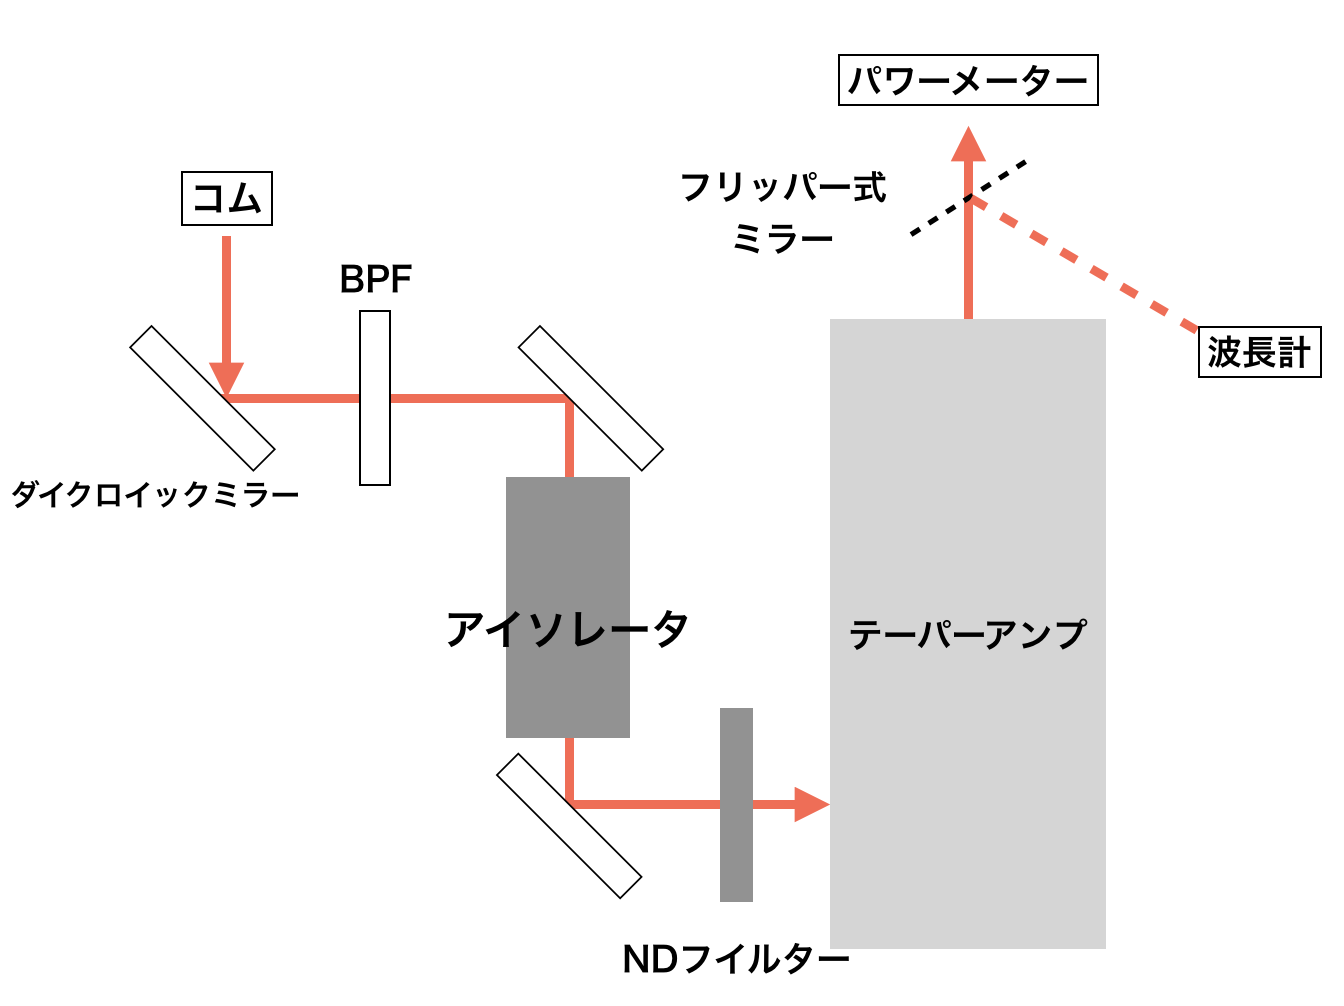
\includegraphics[keepaspectratio,  scale=0.35,  angle=0]
          {figures/chapter4/astro_amp_diagram_isolator.png}
          \caption{繰り返し周波数$1.6$ GHzのコムの$766$ nm付近の光を増幅し、TAによる利得の印加電流依存性を測定した際の光学系。}
          \label{astro_amp_diagram_isolator}
      \end{minipage}
    \end{tabular}
\end{figure}
\begin{figure}[H]
  \centering
    \begin{tabular}{c}
      \begin{minipage}{1\hsize}
        \centering
          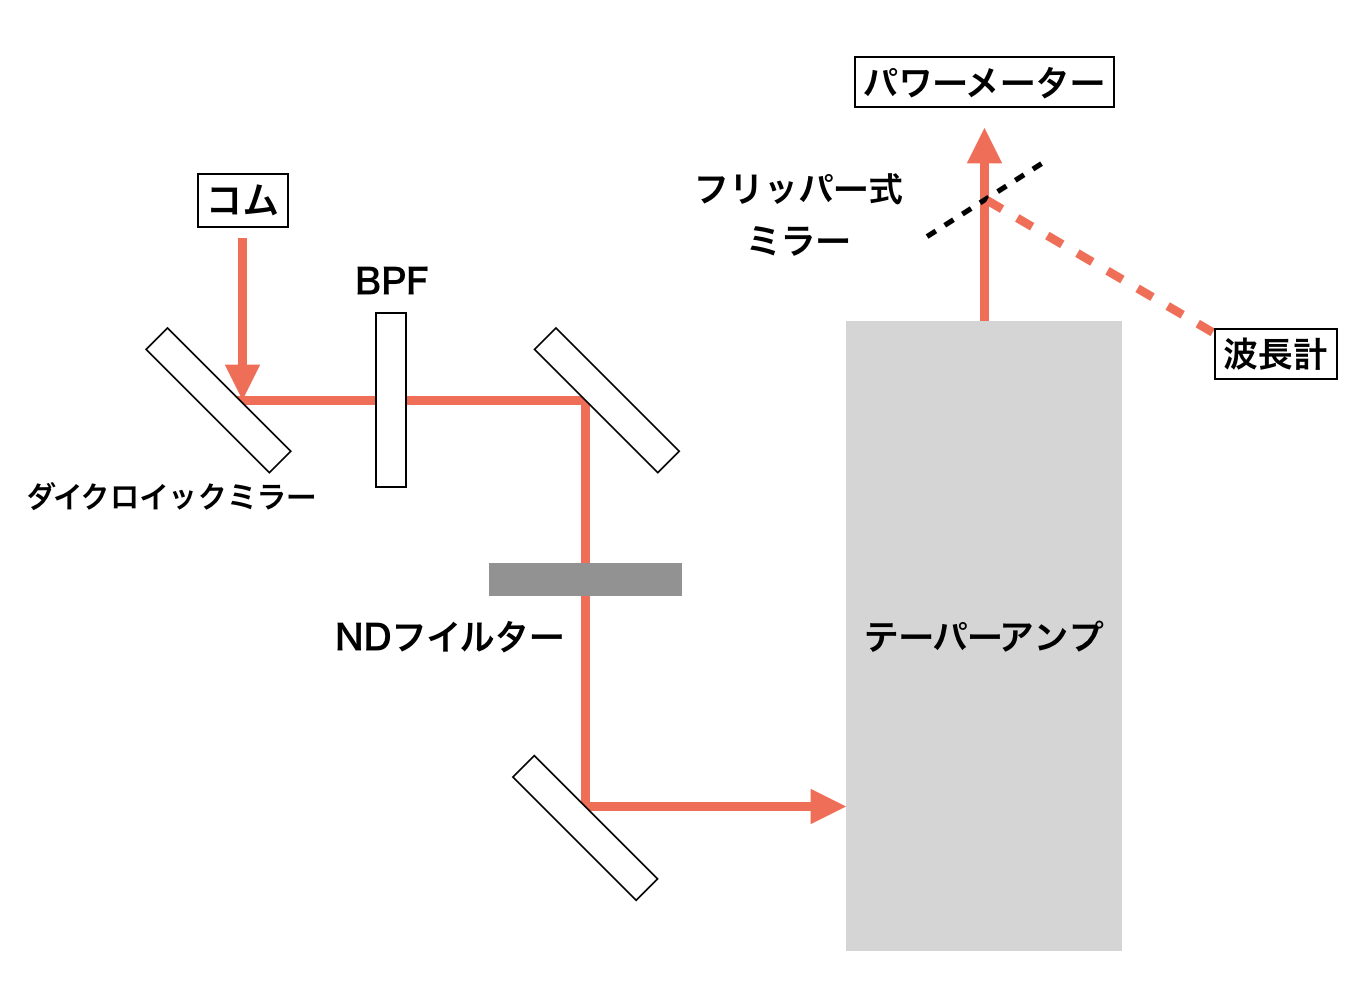
\includegraphics[keepaspectratio,  scale=0.35,  angle=0]
          {figures/chapter4/760_astro_amp_diagram.png}
          \caption{繰り返し周波数$1.6$ GHzのコムの$766$ nm付近の光を増幅し、スレーブパワーのマスターパワー依存性を測定した際の光学系。}
          \label{760_astro_amp_diagram}
      \end{minipage}
    \end{tabular}
\end{figure}

\subsection{測定結果}
TAによる利得の印加電流依存性については、図\ref{current-gain_astro766}のようなデータが得られた。$900$ mA付近と$1200$ mA付近で利得に滑らかでない揺らぎが見られるが、これは測定時にコムの共振器の状態があまり良くなく、マスターパワーが低下してしまったことが原因だと考えられる。\\
(エラーバーを追加)\\
(マスターパワー依存性についてもエラーバーを追加)
\begin{figure}[H]
  \centering
    \begin{tabular}{c}
      \begin{minipage}{1\hsize}
        \centering
          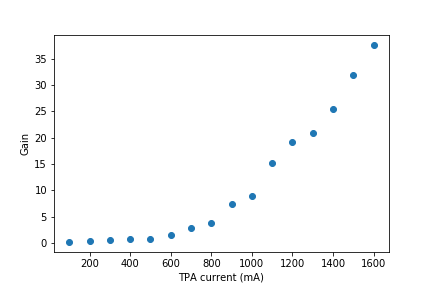
\includegraphics[keepaspectratio,  scale=0.7,  angle=0]
                          {figures/chapter4/current-gain_astro766.png}
                          \caption{TAによる利得の印加電流依存性. $f_\mathrm{rep} = 1.6$ GHzのコムで$766$ nm付近の光をマスターとして使用した。}
                          \label{current-gain_astro766}
      \end{minipage}\\

      \begin{minipage}{1\hsize}
        \centering
          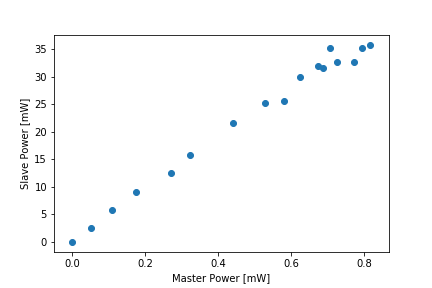
\includegraphics[keepaspectratio,  scale=0.7,  angle=0]
                          {figures/chapter4/astro_seed_dependency760.png}
                          \caption{スレーブパワーのマスターパワー依存性. $f_\mathrm{rep} = 1.6$ GHzのコムで$766$ nm付近の光をマスターとして使用した。}
                          \label{astro_seed_dependency760}
      \end{minipage}

  \end{tabular}
\end{figure}
\newpage
\begin{figure}[H]
  \centering
    \begin{tabular}{c}
      \begin{minipage}{1\hsize}
        \centering
          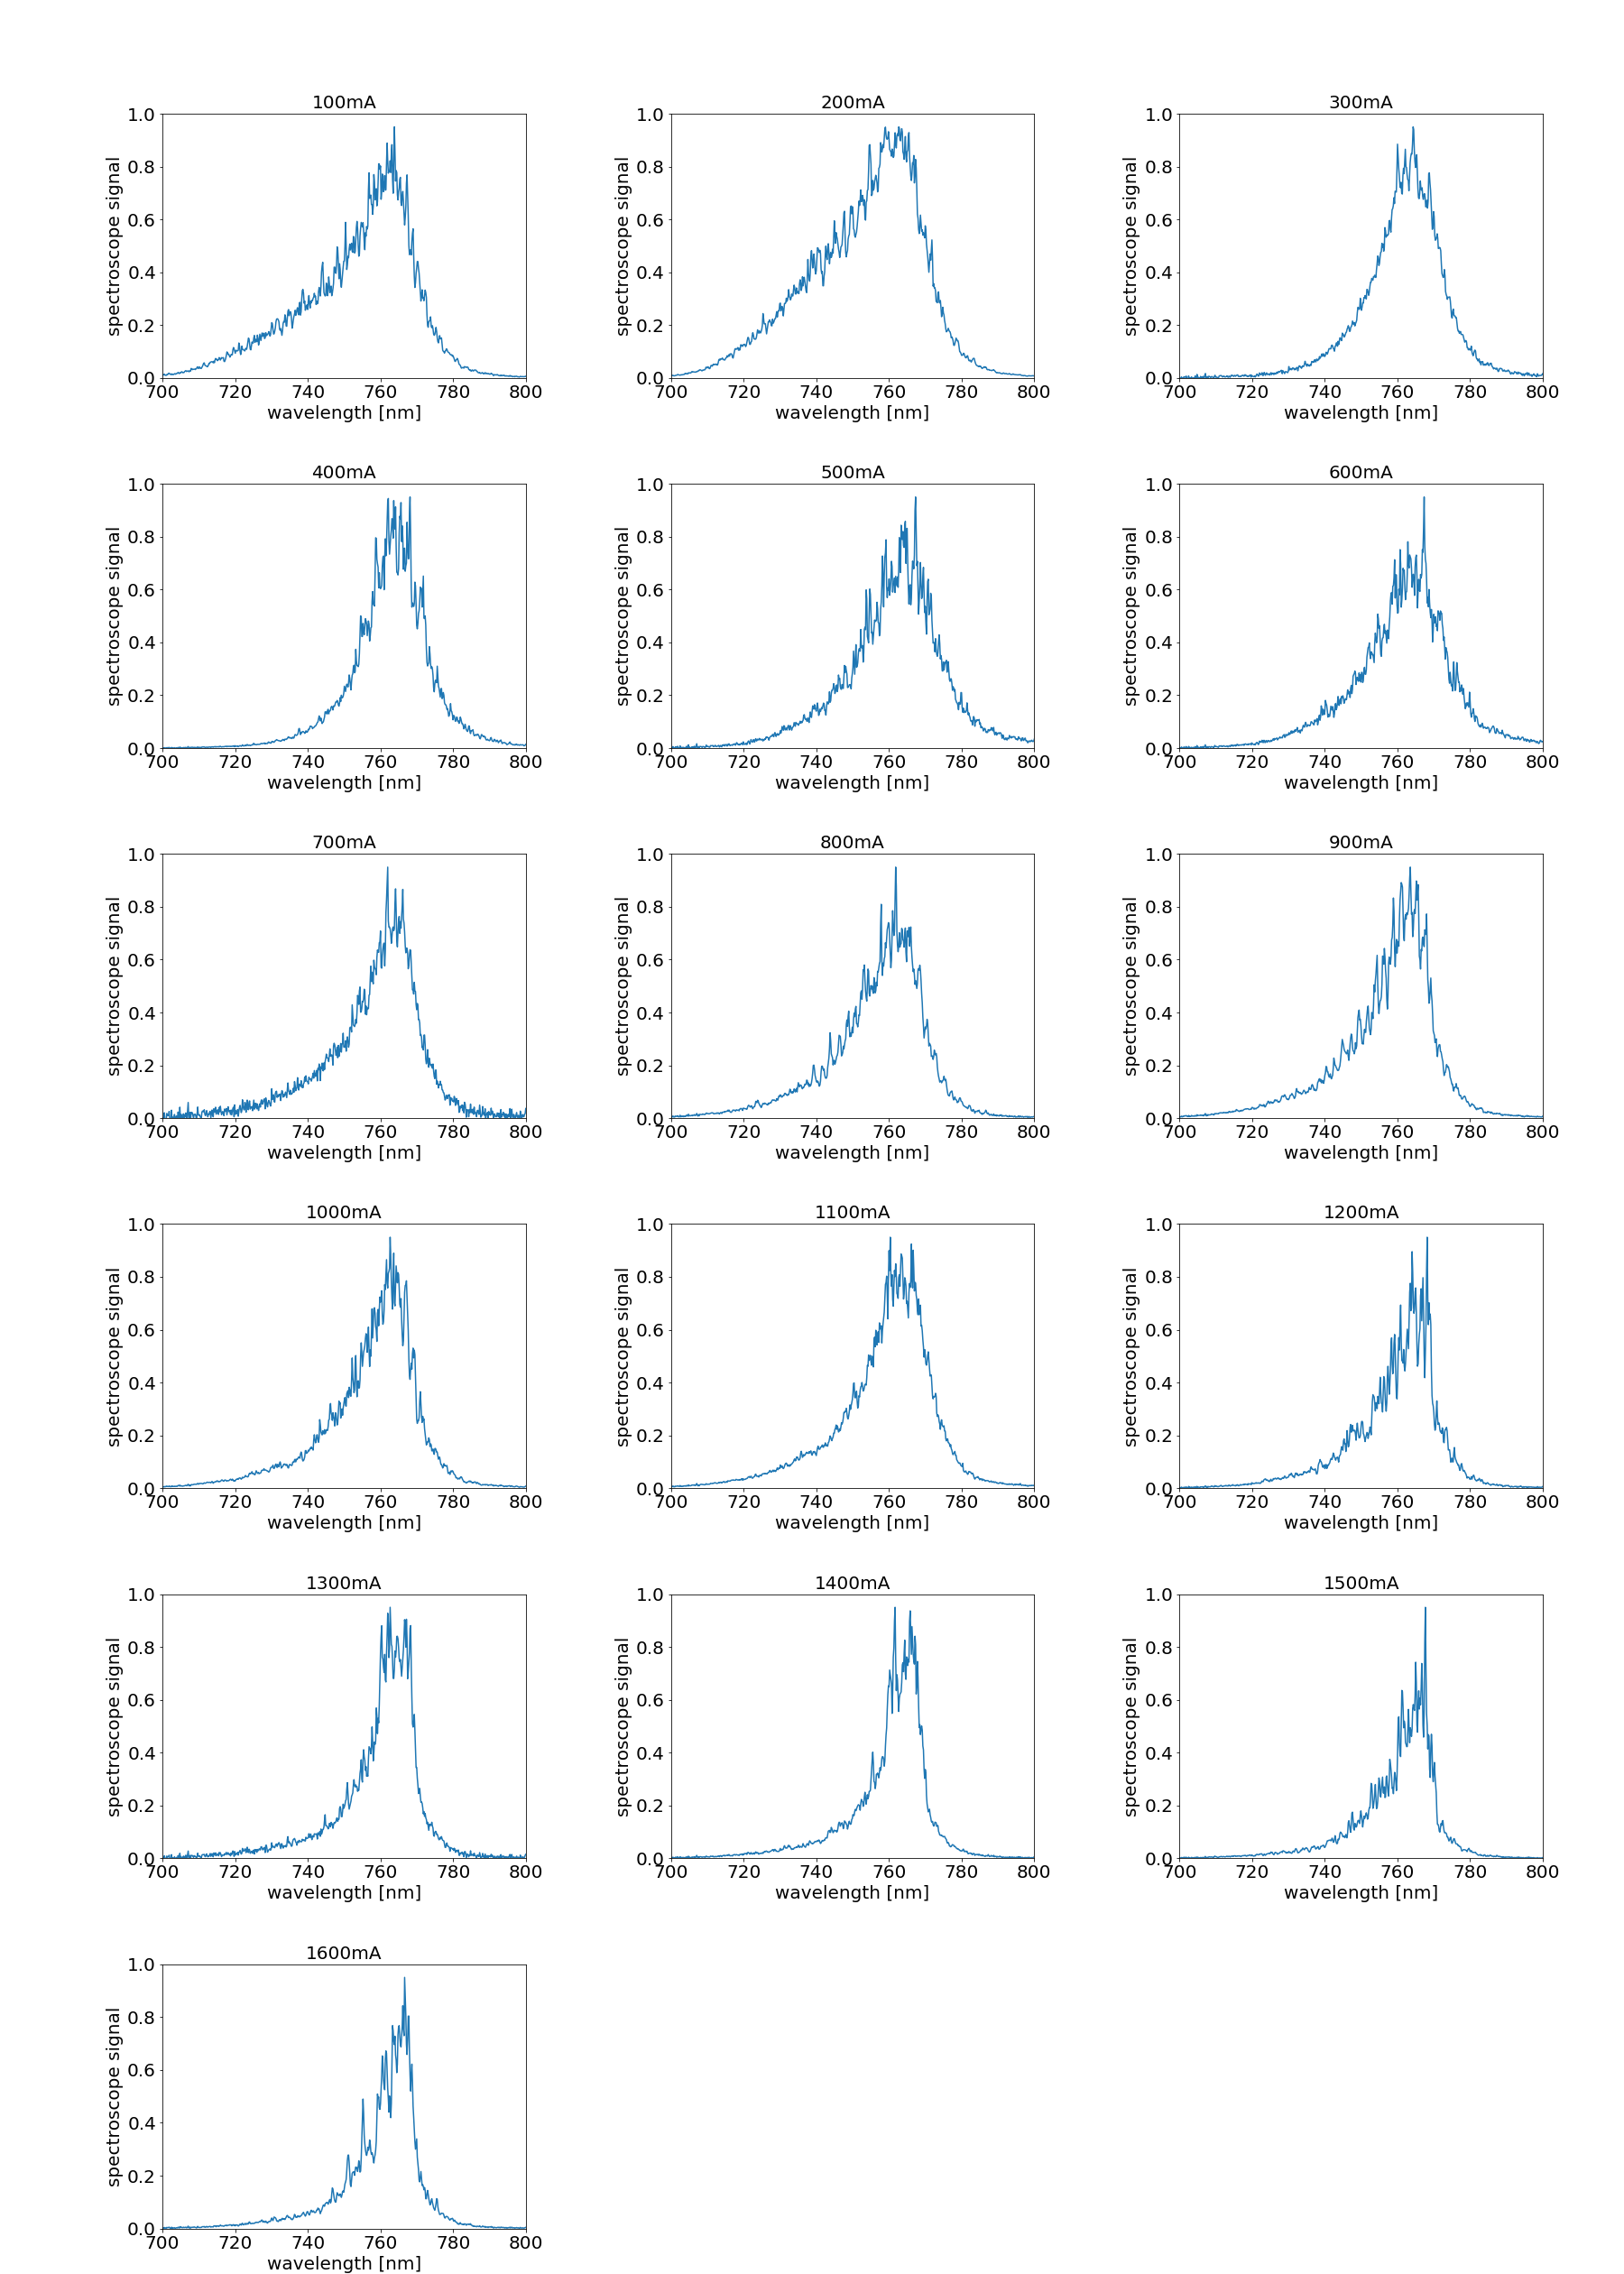
\includegraphics[keepaspectratio,  scale=0.23,  angle=0]
                          {figures/chapter4/760_slave-current_spectrum_astro.png}
                          \caption{スレーブ光のスペクトルのTAの印加電流依存性. $f_\mathrm{rep} = 1.6$ GHzのコムで$766$ nm付近の光をマスターとして使用した。スペクトルの形状を比較するため、分光器の信号の最大値が全てのグラフで同じとなるように規格化を行った。}
                          \label{760_slave-current_spectrum_astro}
      \end{minipage}
  \end{tabular}
\end{figure}

\newpage
\begin{figure}[H]
  \centering
    \begin{tabular}{c}
      \begin{minipage}{1\hsize}
        \centering
          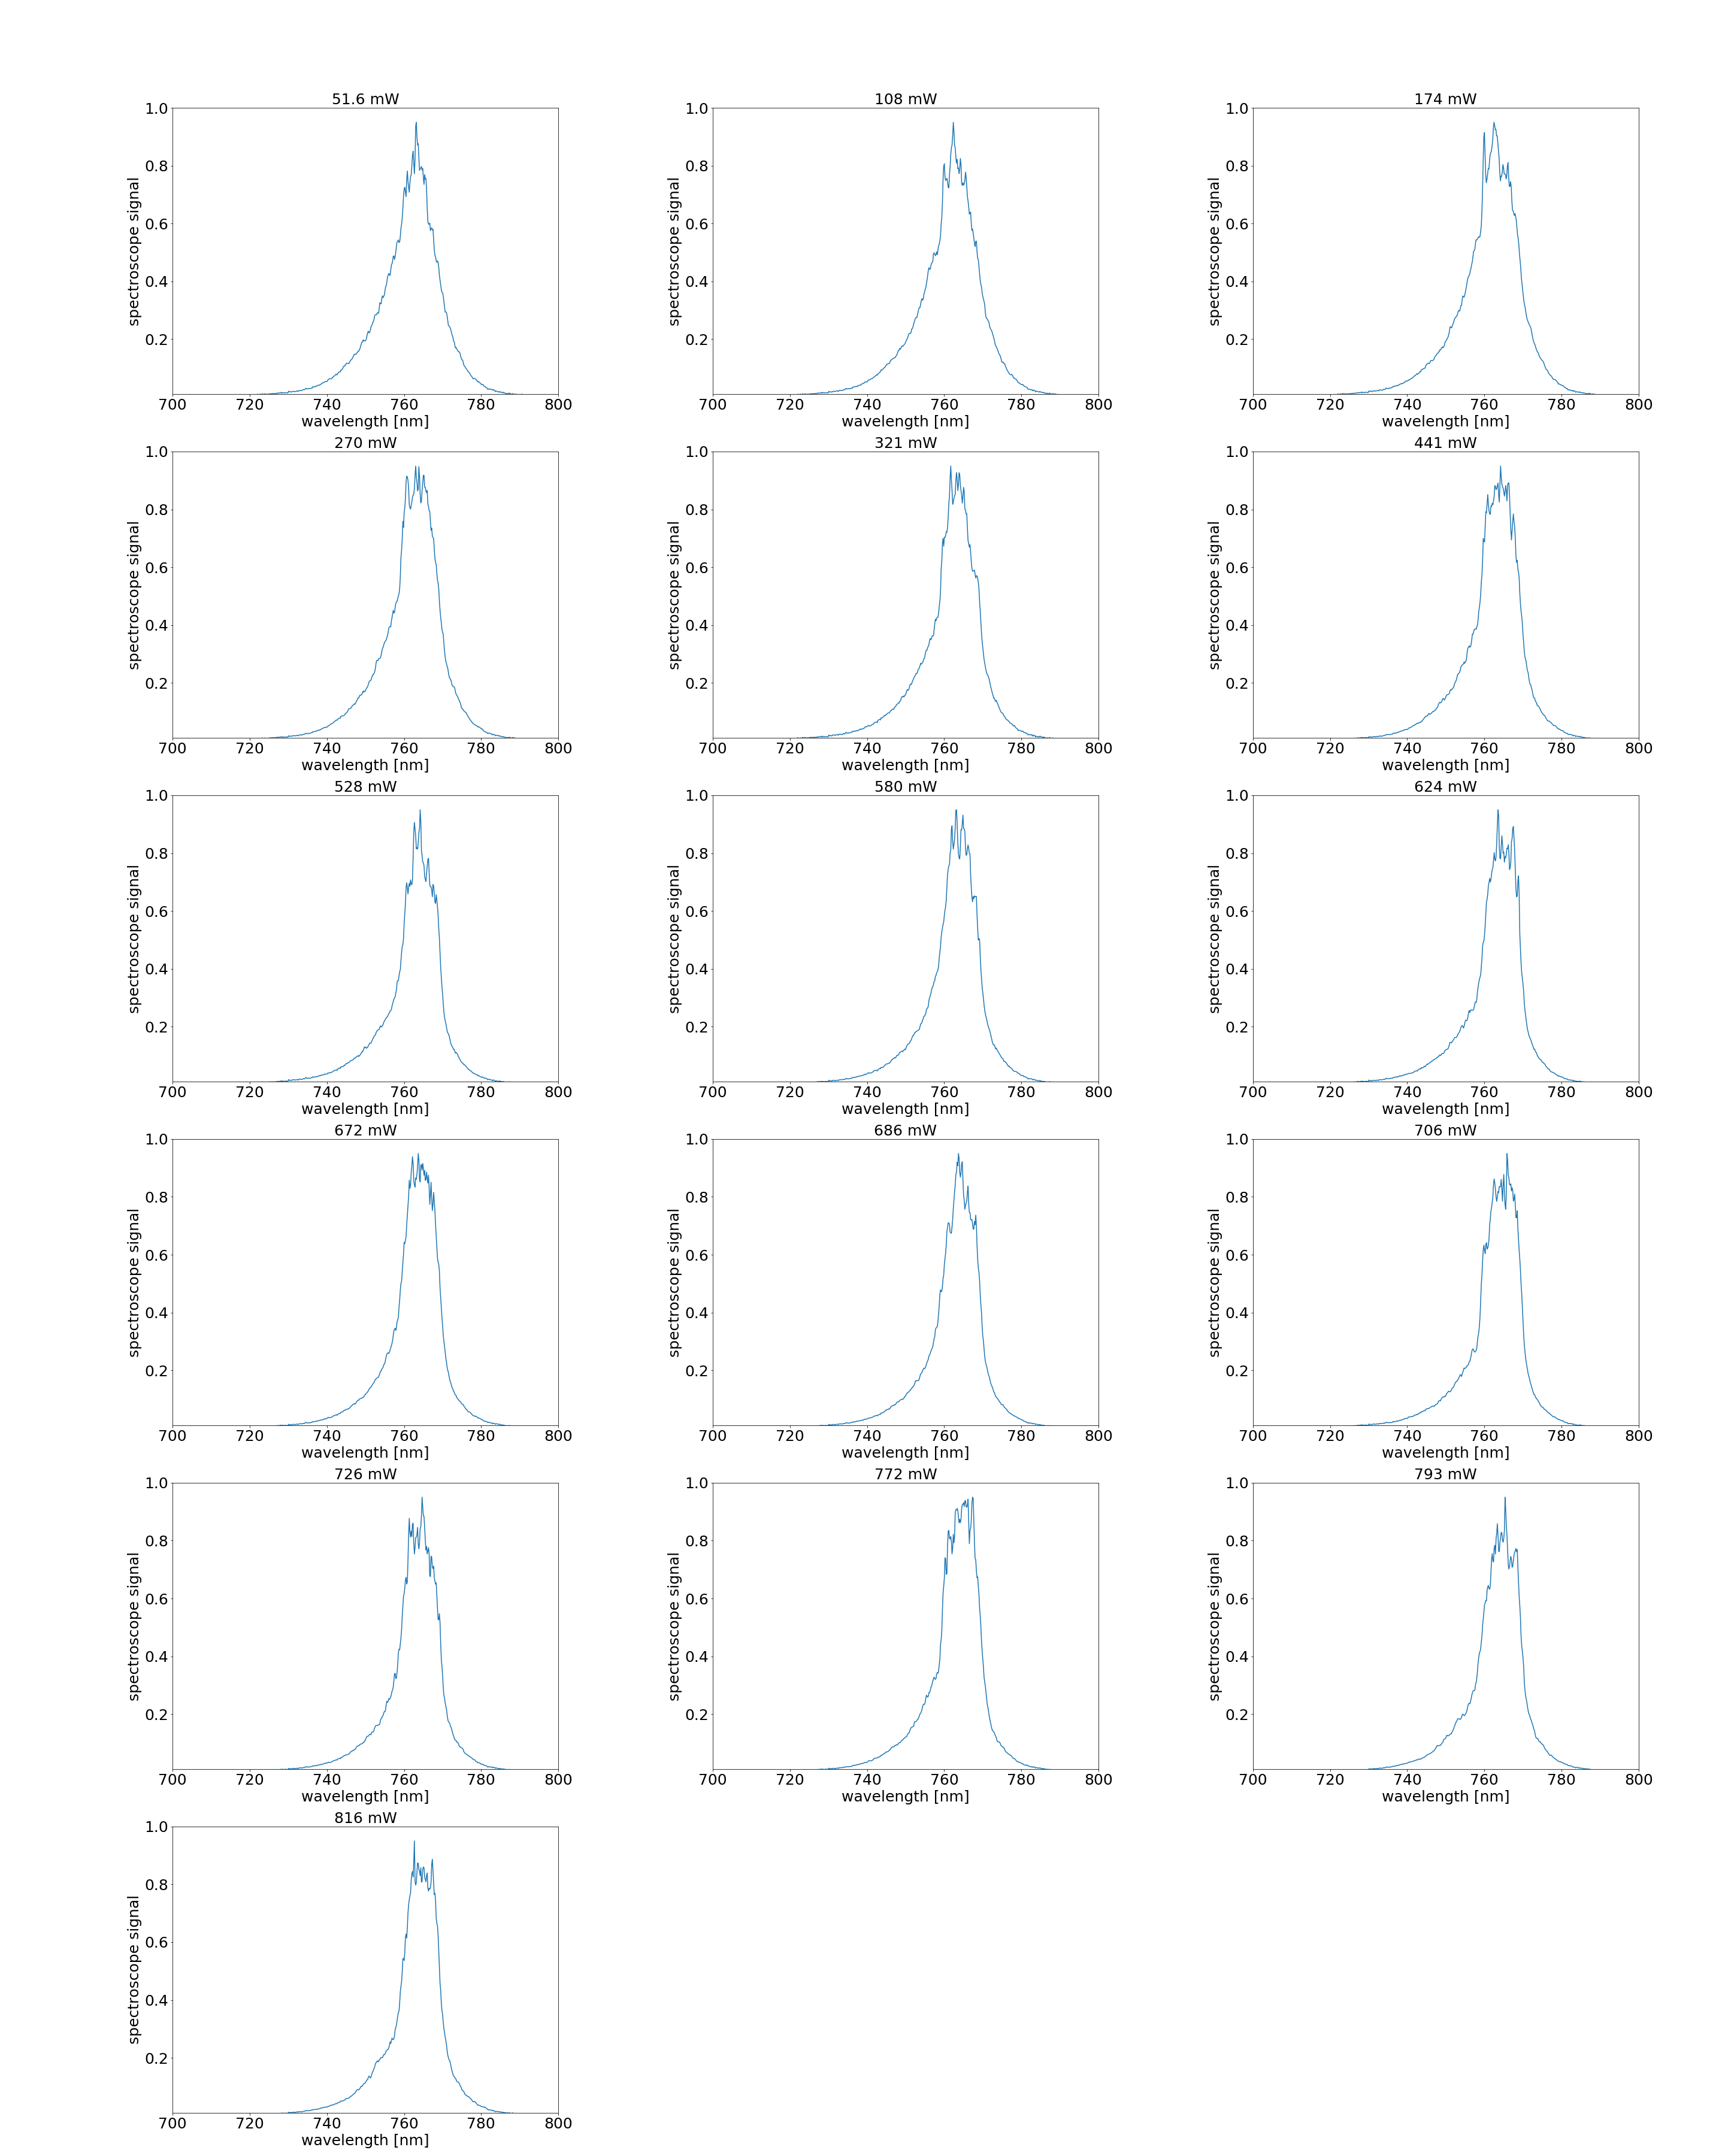
\includegraphics[keepaspectratio,  scale=0.15,  angle=0]
                          {figures/chapter4/astro_TA_output_seed_dependency766.png}
                          \caption{スレーブ光のスペクトルのマスター光のパワー依存性. $f_\mathrm{rep} = 1.6$ GHzのコムで$766$ nm付近の光をマスターとして使用した。スペクトルの形状を比較するため、分光器の信号の最大値が全てのグラフで同じとなるように規格化を行った。}
                          \label{astro_TA_output_seed_dependency766}
      \end{minipage}
  \end{tabular}
\end{figure}

\subsection{繰り返し周波数$120$ MHzのコムの増幅実験との比較}
 スレーブ光強度のマスター光強度依存性を二台のコムで比較すると図\ref{M-S_power-comparison}のようになる。同じマスター光強度で比較すると、繰り返し周波数が$1.6$ GHzのコムのスレーブ光強度が上回っていることがわかる。これは同じ光強度の場合、繰り返し周波数が$120$ MHzのコムでは繰り返し周波数が$1.6$ GHzのコムに比べ一つのパルスに含まれる光子数が多いが、TA内のキャリア数が少ないので誘導放出に使われない光子数が多くなってしまい光が増幅されないことが原因だと考えられる。一方、$1.6$ GHzのコムでは一パルスあたりの光子数が少ないため、無駄になる光子が少なく効率よく増幅することができると考えられる。\\
 図\ref{pulse_power-gain-comparison}は766nm側のコムを増幅した際の利得のパルスエネルギー依存性依存性を二つの繰り返し周波数に応じて比較したものである。繰り返し周波数$120 \mathrm{MHz}$の利得をみると、パルスエネルギーの増加に対して利得が低下していく様子がわかる。これは、各パルスに含まれる光子数に対して励起状態にあるキャリア数が足りておらずパルスエネルギーの増加に対して利得を保てていないことを表していると考えられる。それに対し、繰り返し周波数$1.6 \mathrm{GHz}$のコムの利得は$120$ MHzのコムの利得を下回っている。これはパルスの時間間隔が$630$ ps程度で短く、十分な反転分布が励起されていないことが原因ではないかと考えられる。\\
 また、二台のコムにおける利得の印加電流依存性を比較すると、図\ref{TA_cuurent-gain_comparison}のようなグラフが得られる。繰り返し周波数の高い$f_\mathrm{rep} = 1.6$ GHzのコムは同じ平均パワーの$f_\mathrm{rep} = 120$ MHzよりも高い利得を得ていることが分かる。前述のような理由からであると考えられる。

\begin{figure}[htpb]
  \centering
    \begin{tabular}{c}

%----- 写真 -----


%----- PD Signal -----

      \begin{minipage}{1\hsize}
        \centering
          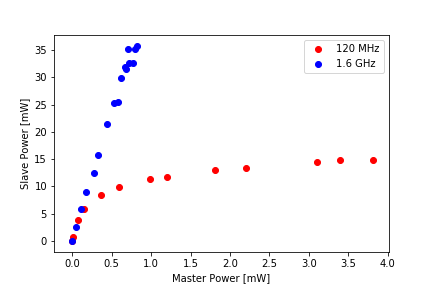
\includegraphics[keepaspectratio,  scale=0.7,  angle=0]
                      {figures/chapter4/M-S_power_comparison.png}
                      \caption{二台のコムにおけるスレーブ光パワーのマスター光パワー依存性の比較}
                      \label{M-S_power-comparison}
      \end{minipage}\\

      \begin{minipage}{1\hsize}
        \centering
          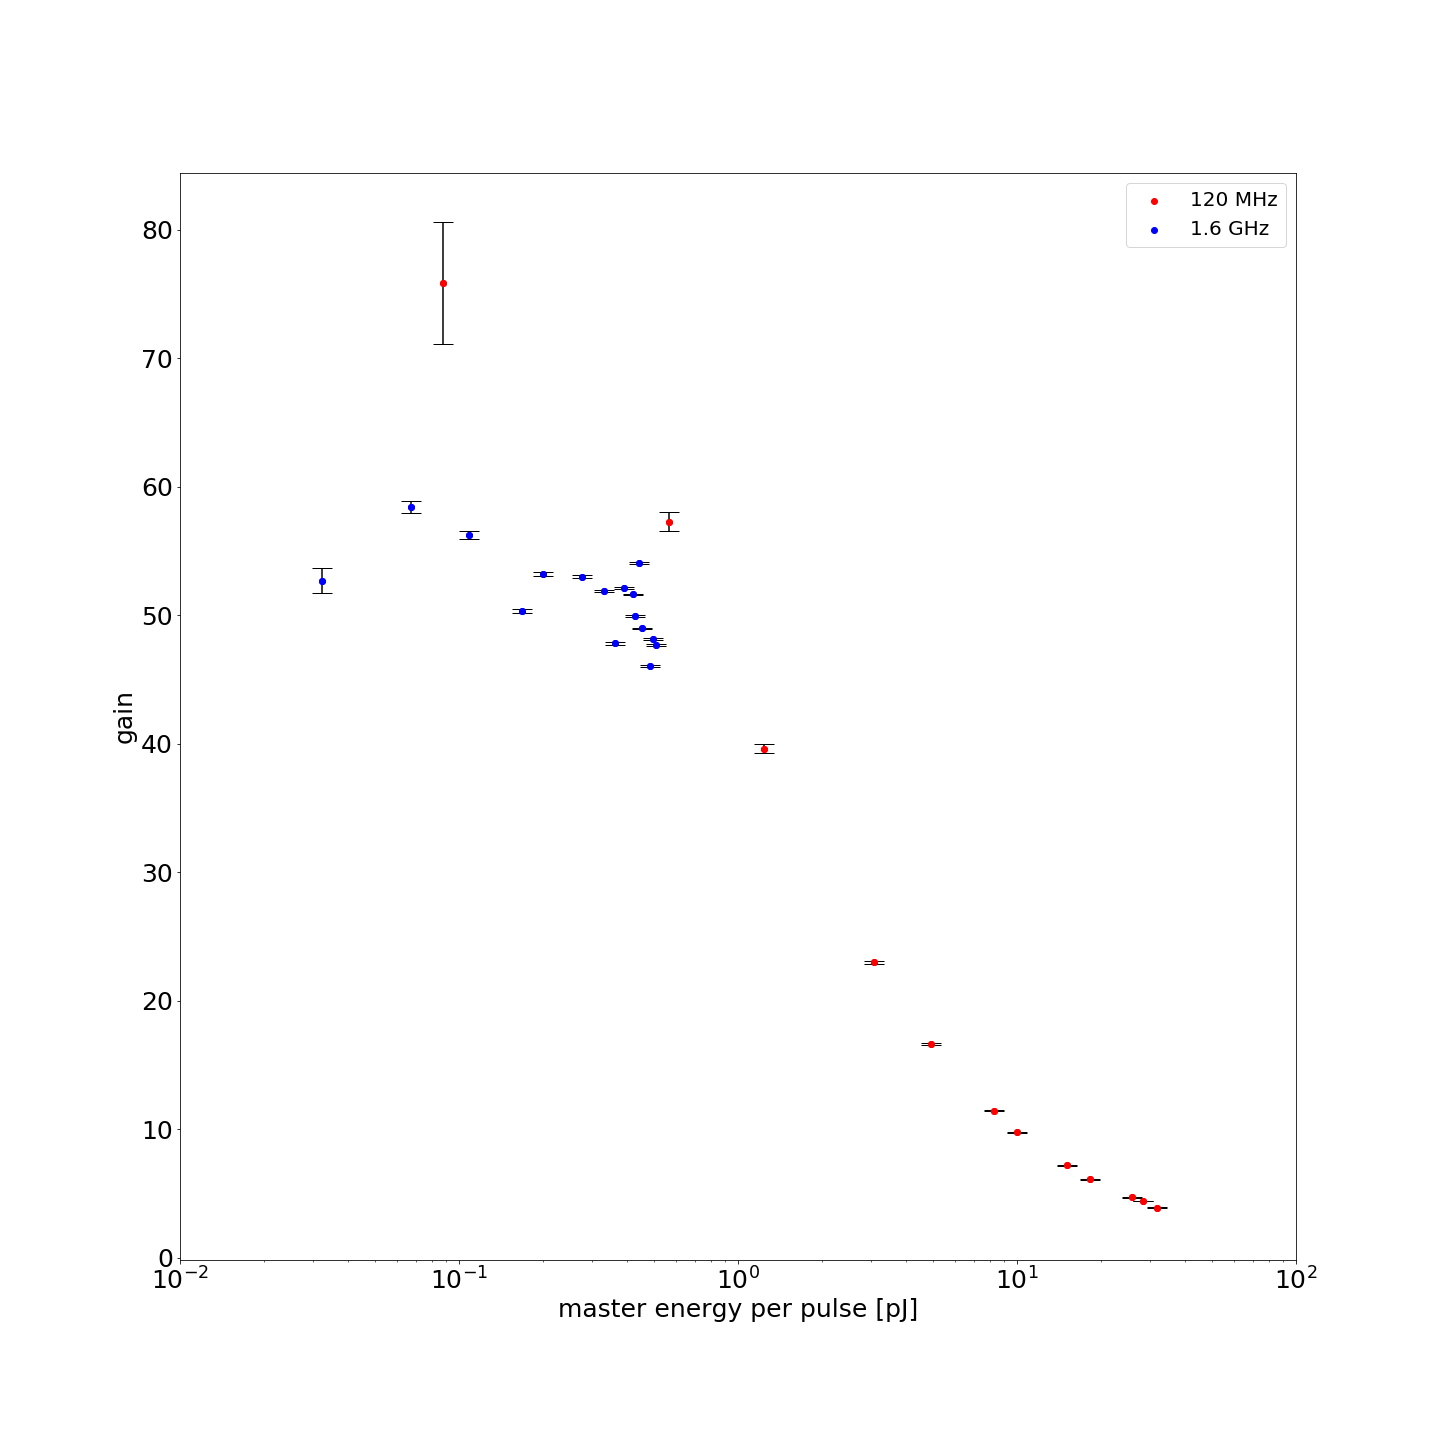
\includegraphics[keepaspectratio,  scale=0.25,  angle=0]
                          {figures/chapter4/pulse_power-gain-comparison_errorbar.png}
                          \caption{二台のコムにおけるTAの利得のパルスエネルギー依存性の比較。エラーバーは測定時の有効数字の最終桁に起因する不確かさを示す。}
                          \label{pulse_power-gain-comparison}
      \end{minipage}
    \end{tabular}
\end{figure}

\newpage
\begin{figure}[H]
  \centering
    \begin{tabular}{c}
      \begin{minipage}{1\hsize}
        \centering
          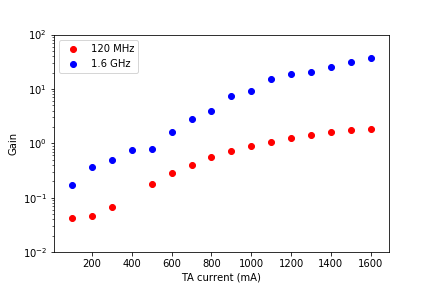
\includegraphics[keepaspectratio,  scale=0.8,  angle=0]
          {figures/chapter4/TA_cuurent-gain_comparison.png}
          \caption{二台のコムにおけるTAの利得の印加電流依存性の比較}
          \label{TA_cuurent-gain_comparison}
      \end{minipage}
    \end{tabular}
\end{figure}
\newpage
\section{$890$ nm用テーパーアンプのチップマウンターの組み立て}
 今回の実験では、Cs原子のレーザー冷却に必要なパワーを得るためにTAを用いた。光周波数コムのから$760 \mathrm{nm}$付近の波長と$890 \mathrm{nm}$付近の波長を切り出し増幅した。$890 \mathrm{nm}$側の増幅に用いるTAのチップのマウンターに関しては、設計と組み立てを行った。TAのチップはeagleyard社のEYP-TPA-0915-01500-3006-CMT03-0000を用いた。TAのチップの構造は図\ref{TA_chip_ds}のようになっている。\\
\begin{figure}[htbp]
 \begin{center}
  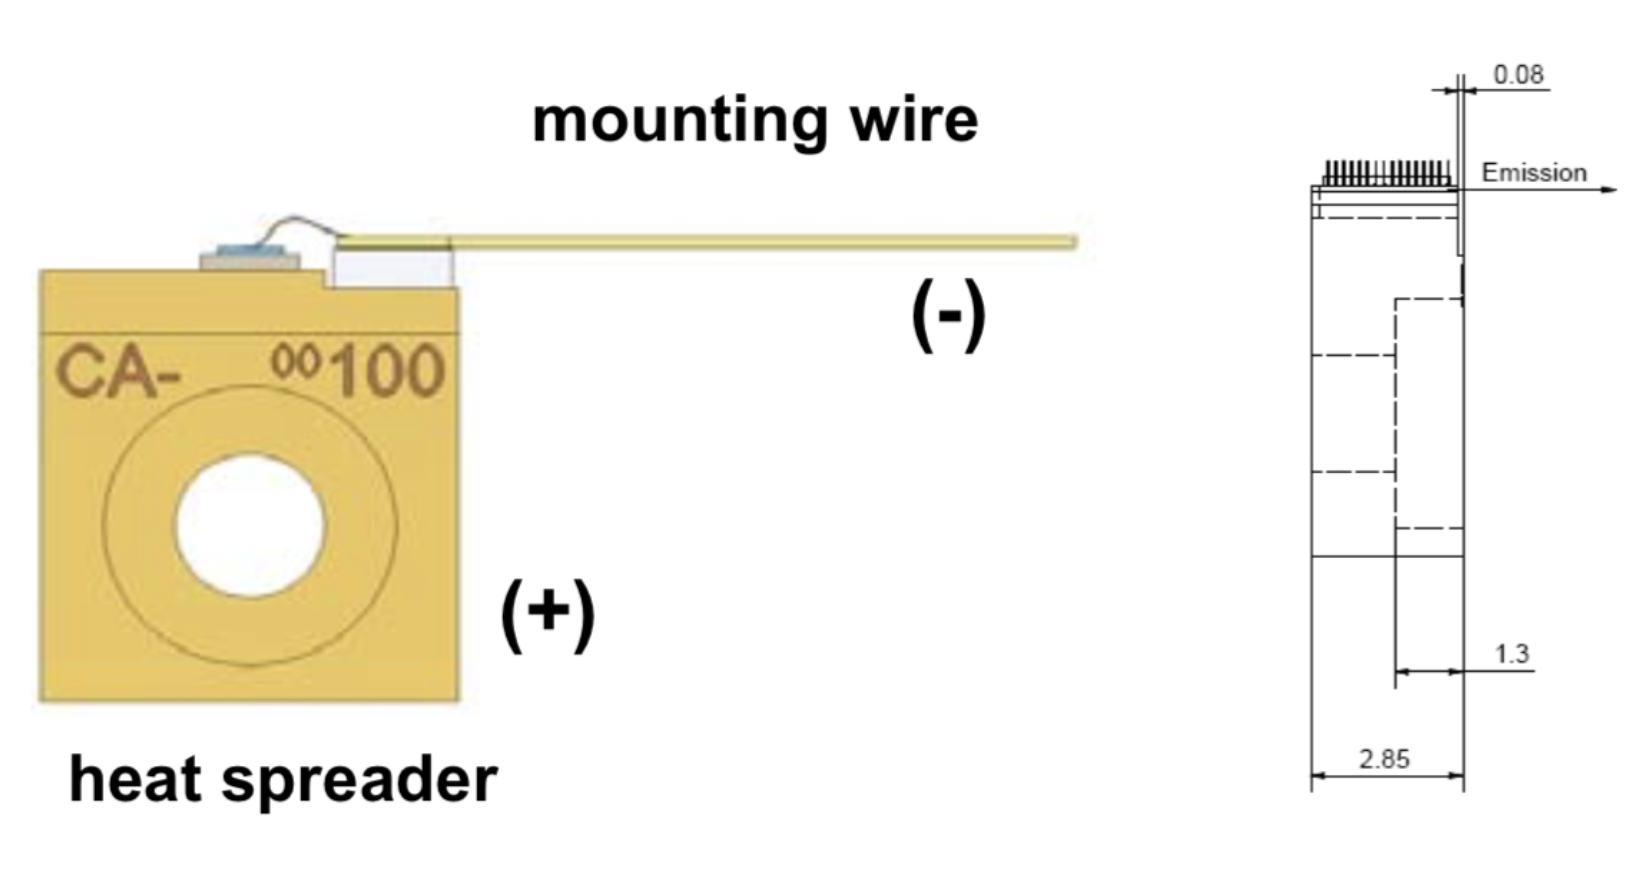
\includegraphics[width=70mm]{figures/chapter4/TA_chip_ds.png}
\end{center}
 \caption{TAチップの構造図(eagleyard社のデータシートから引用)}
 \label{TA_chip_ds}
\end{figure}
 TAチップのマウンターの構造は図\ref{TA_mounter_photo_comments},\ref{TA_mounter_structure}のようになっている。ただし、TAチップの入力光をマスター光、出力光をスレーブ光と呼ぶ。TAチップは銅のブロックにコリメーションレンズ2枚と共に取り付けられており、そこに温度センサーと直流電源からのSMAケーブルが繋がっている。この銅製のブロックをアルミニウム製のブロックを介して光学定盤に固定している。二つのブロックの間にペルチェ素子を挟み、温度を制御している。なお、レンズのマウンターにはアルミニウムを使用している。

\begin{figure}[htpb]
  \centering
    \begin{tabular}{c}

%----- TAチップマウンターの概観 -----

      \begin{minipage}{0.50\hsize}
        \centering
          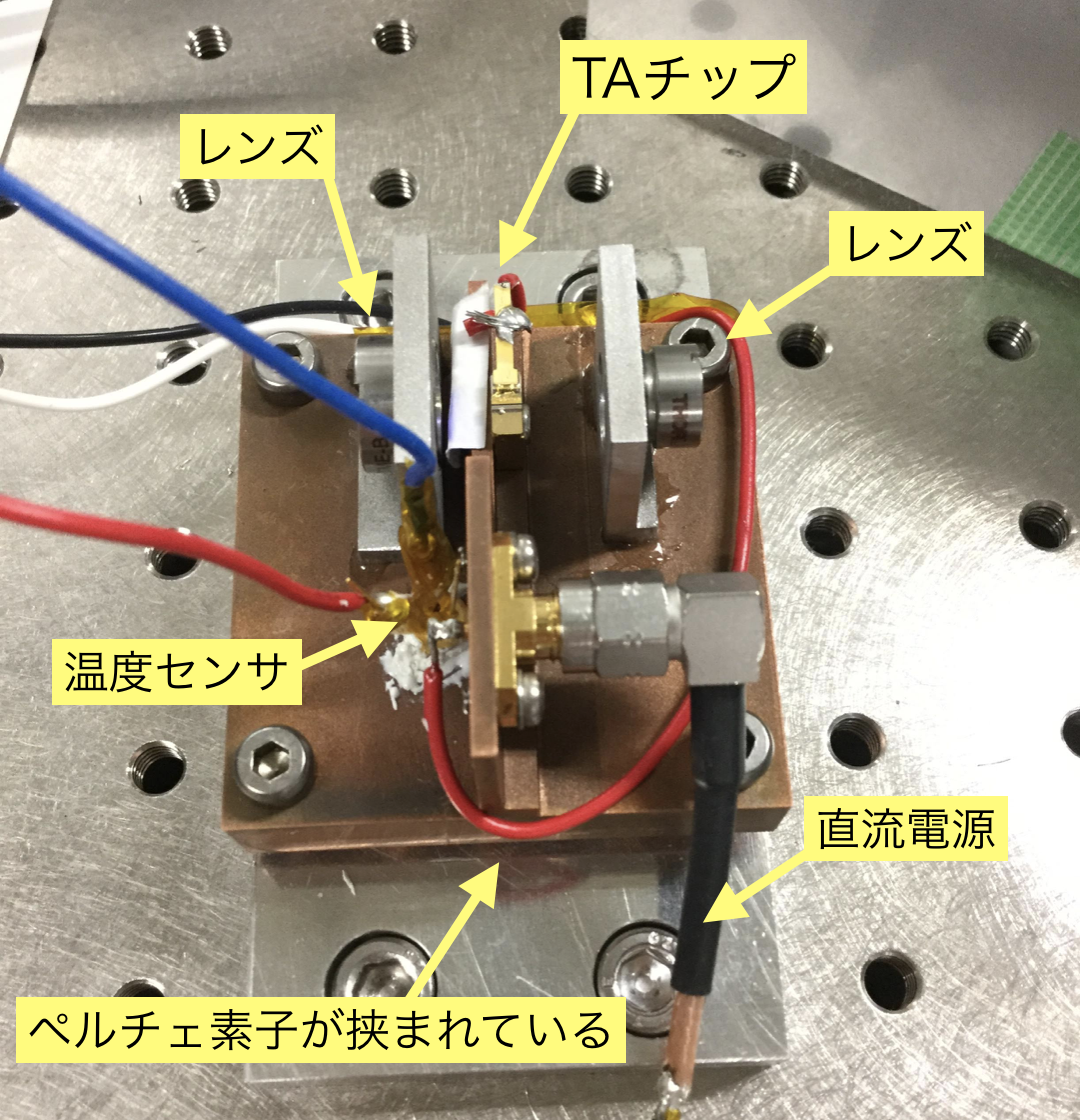
\includegraphics[keepaspectratio,  scale=0.30,  angle=0]
                          {figures/chapter4/TA_mounter_photo_comments.png}
                          \caption{TAチップマウンターの概観}
                          \label{TA_mounter_photo_comments}
      \end{minipage}
%----- TAチップマウンターの構造図 -----

      \begin{minipage}{0.50\hsize}
        \centering
          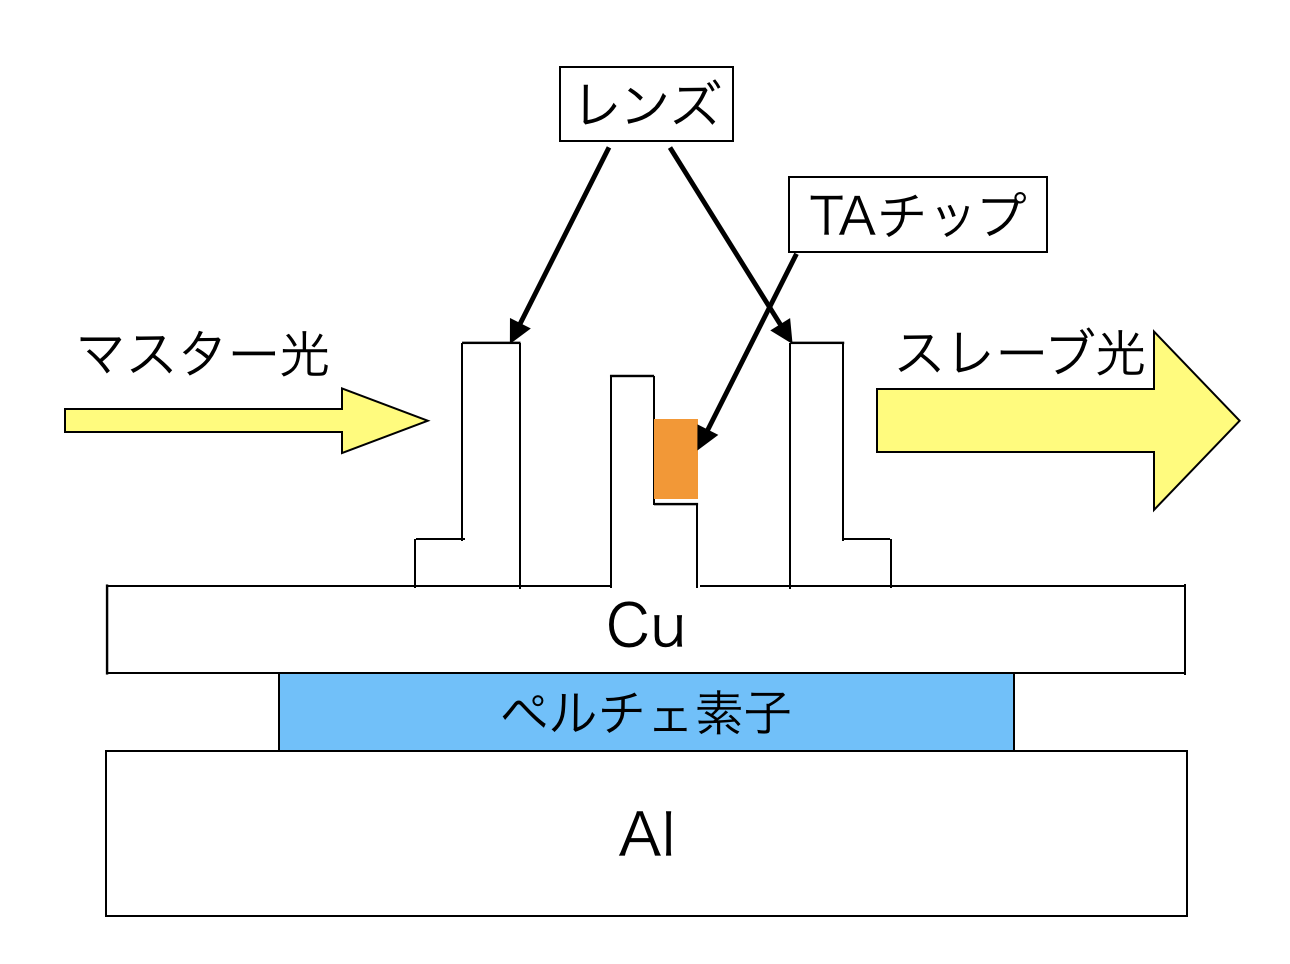
\includegraphics[keepaspectratio,  scale=0.35,  angle=0]
                          {figures/chapter4/TA_mounter_structure.png}
                          \caption{TAチップマウンターの構造図}
                          \label{TA_mounter_structure}
      \end{minipage}

    \end{tabular}
\end{figure}
\newpage
 なお、実際に使用する際には、図\ref{TA_case}のようにアクリルボードでケースを作り使用した。 また、スレーブ光の形状は光の回折の効果から楕円状になっているため、垂直方向のコリメーションを銅ブロック状のレンズで行い、水平方向のコリメーションを追加のシリンドリカルレンズで行う必要がある。\\
\begin{figure}[htbp]
 \begin{center}
  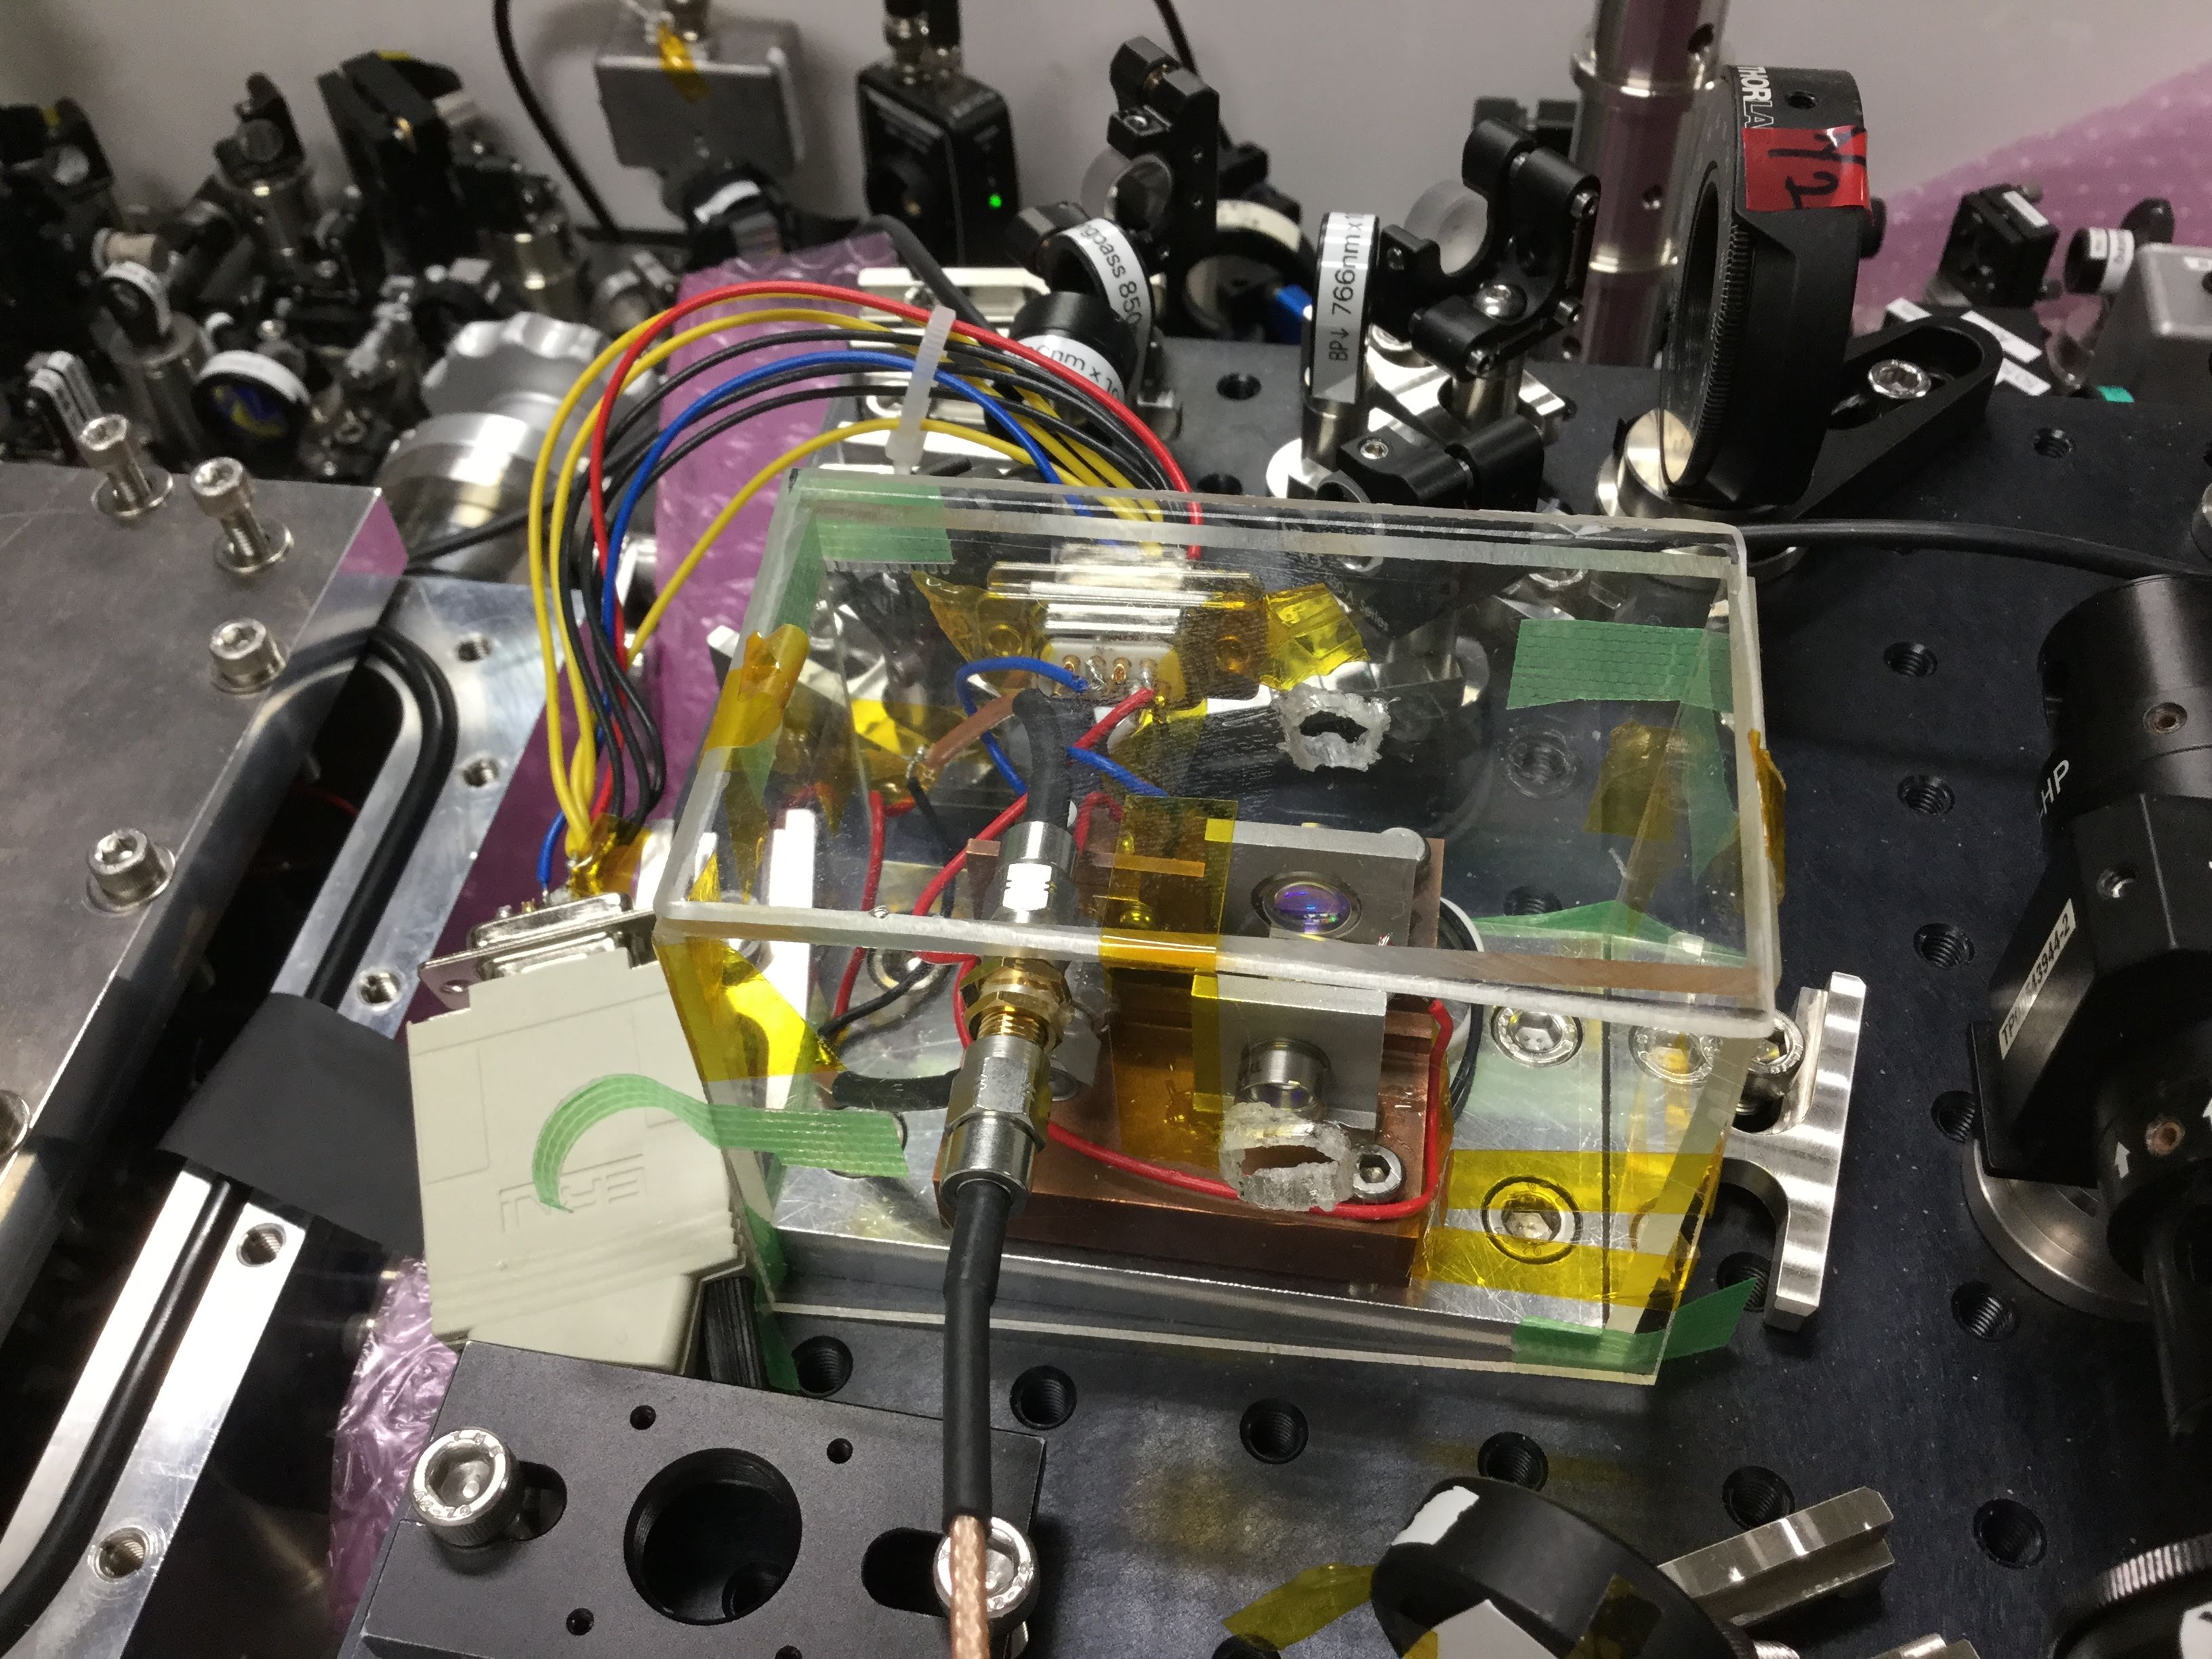
\includegraphics[width=75mm]{figures/chapter4/TA_case.jpg}
\end{center}
 \caption{実際に使用時のTAの様子}
 \label{TA_case}
\end{figure}

\section{繰り返し周波数$1.6$ GHzのコムの$890$ nm付近の増幅}
\subsection{測定手法}
 自作したTAで繰り返し周波数が$1.6$ GHzのコムの、$890$ nmを中心波長とする幅$10$ nmのBPFを通過した光を増幅させた。その際の光学系は図\ref{890_astro_amp_diagram}に示した。マスター光のパワーが一定の下でスレーブ光のパワーの電流依存性の測定を行った。また、TAの印加電流$1.95$ Aの下でスレーブ光のパワーのマスター光のパワーの依存性を測定した。測定の際にはTAのチップの温度が安定するように、マスター光のパワーが最大の点から測定を開始し、パワーを順に下げていくように測定を行った。

\begin{figure}[H]
  \centering
    \begin{tabular}{c}
      \begin{minipage}{1\hsize}
        \centering
          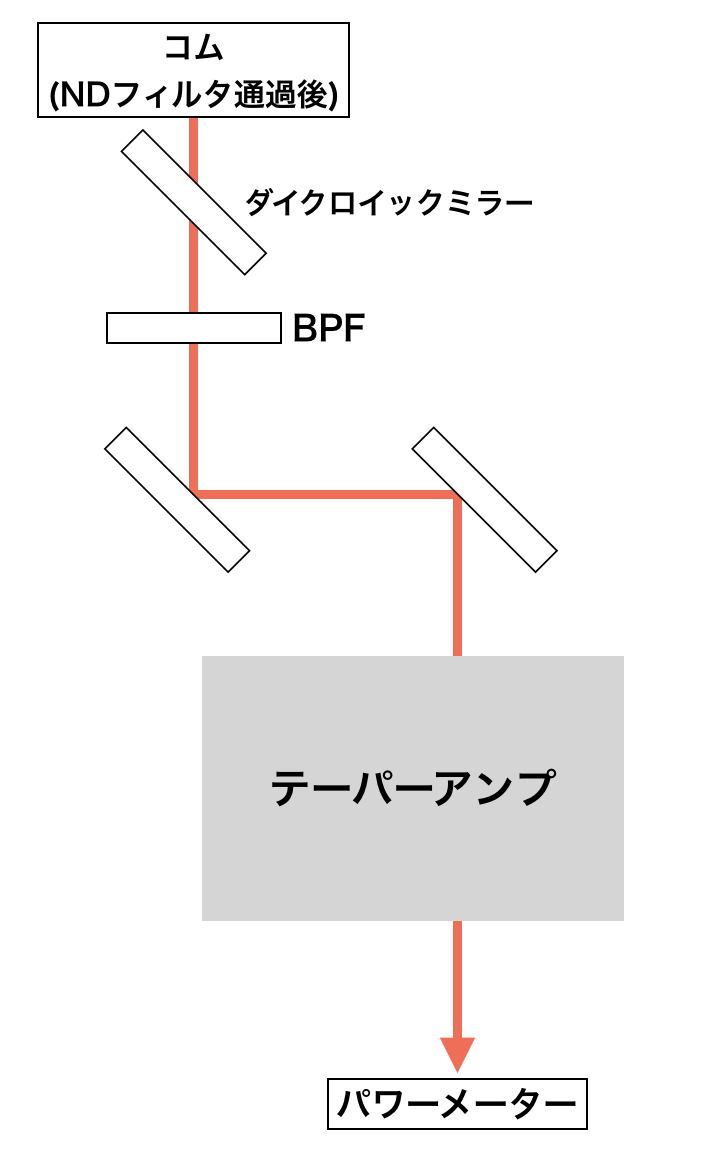
\includegraphics[keepaspectratio,  scale=0.4,  angle=0]
          {figures/chapter4/890_astro_amp_diagram.png}
          \caption{繰り返し周波数$1.6$ GHzのコムの$890$ nm付近の光を増幅した際の光学系}
          \label{890_astro_amp_diagram}
      \end{minipage}
    \end{tabular}
\end{figure}

\subsection{測定結果}
結果を、図\ref{TA_power-current_3A_astro}, \ref{890TPA_power_dependence_0117}に示す。

\begin{figure}[H]
  \centering
    \begin{tabular}{c}

%----- 写真 -----

      \begin{minipage}{0.50\hsize}
        \centering
          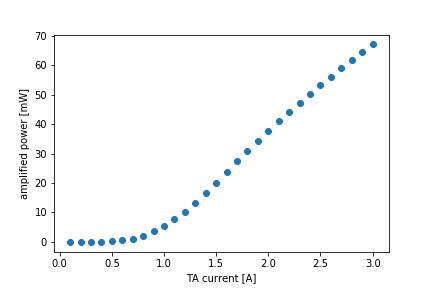
\includegraphics[keepaspectratio,  scale=0.50,  angle=0]
                          {figures/chapter4/TA_power-current_3A_astro.png}
                          \caption{890nm側の繰り返し周波数$1.6$ GHzでのTAのスレーブ光パワーの電流依存性}
                          \label{TA_power-current_3A_astro}
      \end{minipage}

%----- PD Signal -----

      \begin{minipage}{0.50\hsize}
        \centering
          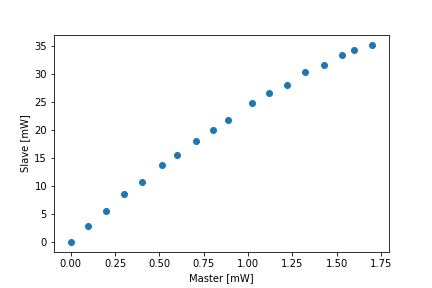
\includegraphics[keepaspectratio,  scale=0.5,  angle=0]
                          {figures/chapter4/890TPA_power_dependence_0117.png}
                          \caption{890nm側の繰り返し周波数$1.6$ GHzでのTAのスレーブ光パワーのマスター光強度依存性}
                          \label{890TPA_power_dependence_0117}
      \end{minipage} \\

    \end{tabular}
\end{figure}


\section{ダブルパスでの増幅実験}

TAは通常ゲイン領域が細い方からマスター光を入射し、ゲイン領域の広い方からスレーブ光を出力するという使用法をする。しかし、通常の出力側からマスター光を入射し通常の入力側から出た光をミラーで打ち返し再度通常の入力側に光を入射させ、二度ゲイン領域を通過させ増幅するという手法がある。この光学系の配置をダブルパスといい、これに対して通常の配置をシングルパスと呼ぶことがある。ダブルパスでのcwレーザーのTAの増幅の振る舞いについては過去の研究\cite{doi:10.1063/1.3501966}があり、通常cw光でTAを飽和させるには数十ワットのマスター光が必要となるが、ダブルパスの場合だと$200 \mathrm{\mu W}$のマスター光で飽和させることが出来ることが分かっている。また、スペクトルの面でもキャリアの周波数的に幅の広い自然放出が抑えられることが分かっている。このように、ダブルパスによるメリットは多いが光周波数コムの増幅にダブルパスを用いている研究はまだない。そのため今回の実験では,繰り返し周波数$1.6$ GHzの$761$ nmから$771$ nmのコムをダブルパスにより増幅する実験を行った。


\subsection{測定手法}

\begin{figure}[htbp]
 \begin{center}
  \includegraphics[width=120mm]{figures/chapter4/doublepass_photo.png}
\end{center}
 \caption{ダブルパス配置の光学系}
 \label{doublepass_photo}
\end{figure}

\subsection{測定結果}
ダブルパスでの増幅の様子を図\ref{double-pass_I-Gain},\ref{double-pass_I-Slave}に示す。図\ref{double-pass_I-Slave}で示されたスレーブ光のスペクトルをみると印加電流が$930$ mA以上ではスレーブ光がcw的に発振してしまっていることが分かる。これは、マスター光が$116 \mathrm{\mu W}$と小さなパワーしか用意することができなかったため、使用したTAのゲイン特性の偏りからゲインの高い波長で優先的に自然放出の光が増幅されてしまったものが観測されたと考えられる。

\newpage
\begin{figure}[htpb]
  \centering
    \begin{tabular}{c}
      \begin{minipage}{0.50\hsize}
        \centering
          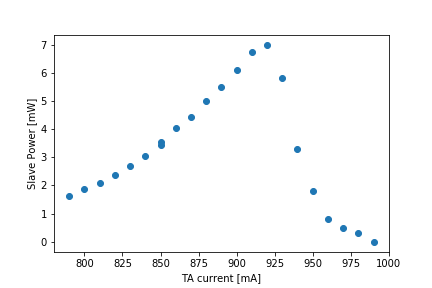
\includegraphics[keepaspectratio,  scale=0.5,  angle=0]
                          {figures/chapter4/double-pass_I-slavepower.png}
                          \caption{ダブルパスでのスレーブ光パワーの印加電流依存性。$f_{\mathrm{rep}} = 1.6$ GHzで$890$ nm付近を増幅した。シード光の平均パワーは$112\ \mu W$である。}
                          \label{double-pass_I-slavepower}
      \end{minipage}
      \begin{minipage}{0.50\hsize}
        \centering
          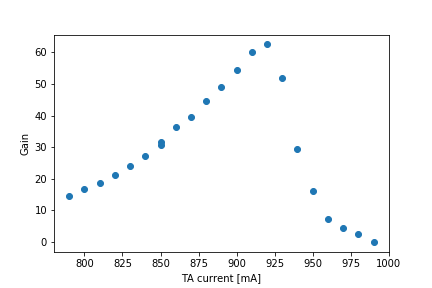
\includegraphics[keepaspectratio,  scale=0.5,  angle=0]
                          {figures/chapter4/double-pass_I-Gain.png}
                          \caption{ダブルパスでの利得の印加電流依存性。測定条件は図\ref{double-pass_I-slavepower}と同じである。}
                          \label{double-pass_I-Gain}
      \end{minipage}\\

      \begin{minipage}{1\hsize}
        \centering
          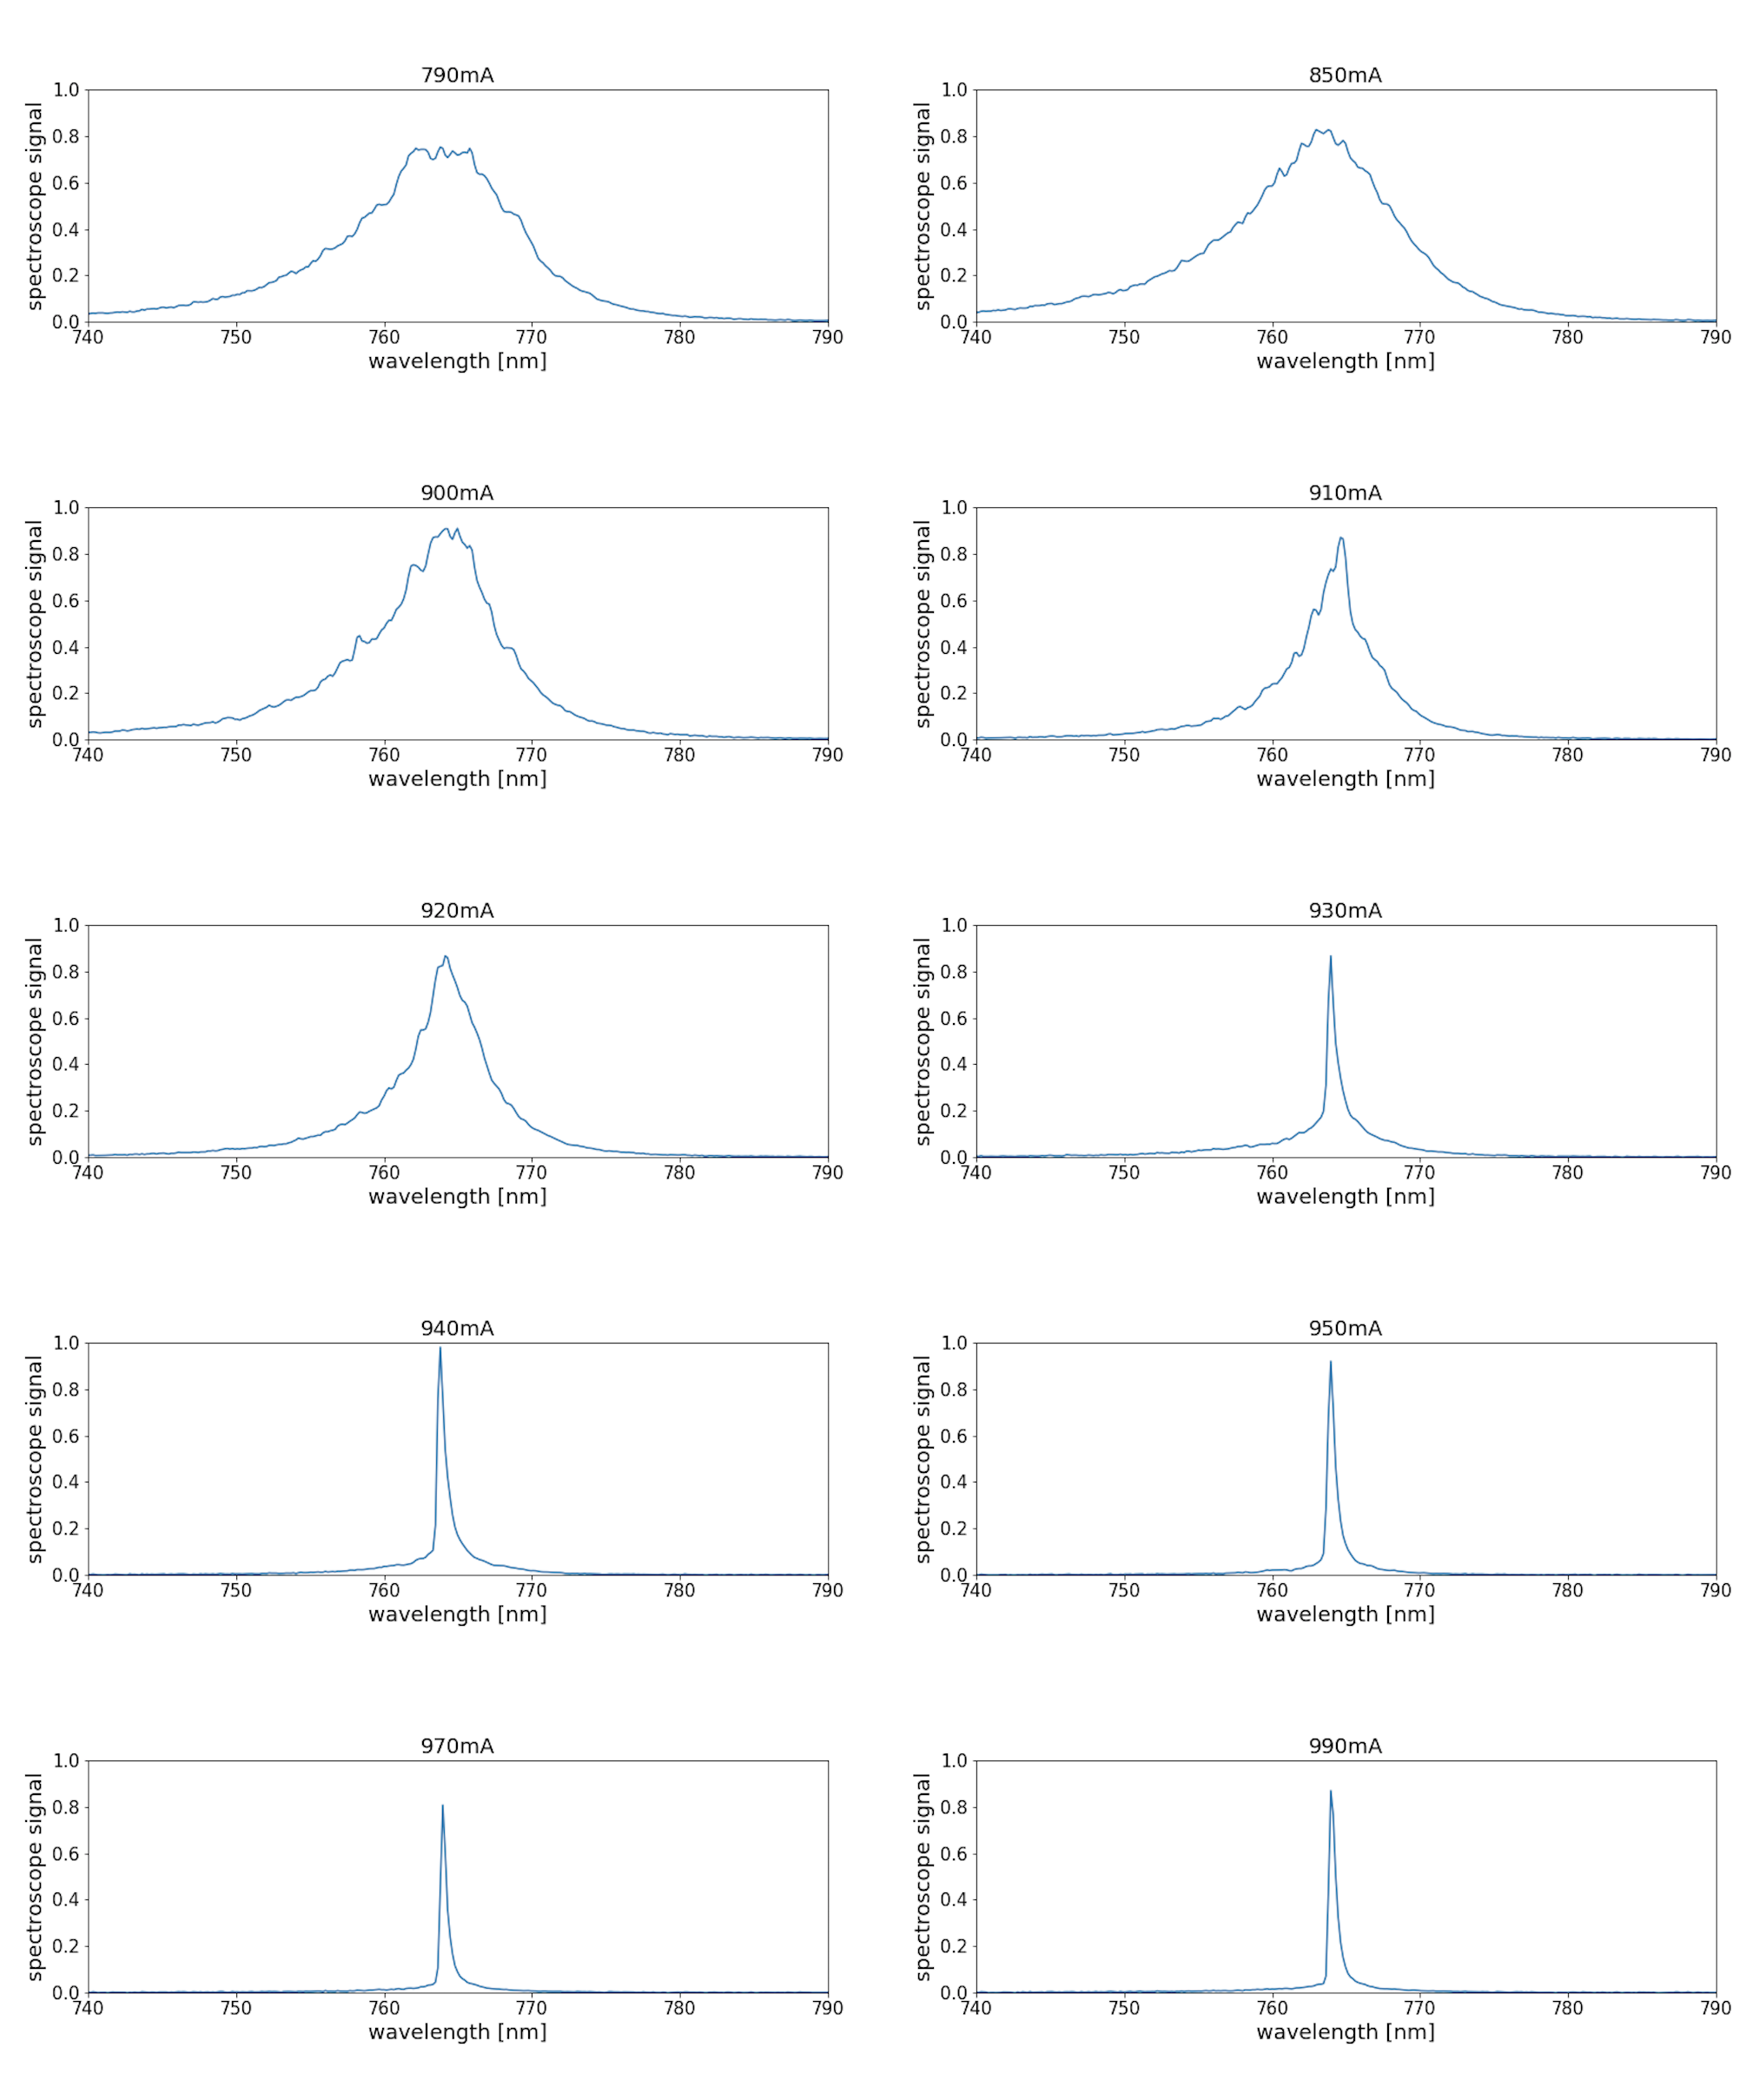
\includegraphics[keepaspectratio,  scale=0.340,  angle=0]
                          {figures/chapter4/double-pass-Slave-Spectrum.png}
                          \caption{ダブルパスでの各印加電流におけるスレーブ光のスペクトル。測定条件は図\ref{double-pass_I-slavepower}と同じである。}
                          \label{double-pass_I-Slave}

      \end{minipage}


    \end{tabular}
\end{figure}
\section{結論}

今回の実験では$766$ nm付近の波長では$35$mW、$890$ nm付近の波長では$70$ mWのパワーを得た。このパワーで二光子冷却の励起効率を見積もると~~であることが分かる。

\bibliography{reference}
\end{document}
